\chapter{Random Variables}\label{S:RandomVariable}
It can be be inconvenient to work with a set of outcomes $\Omega$ upon which arithmetic is not possible.  We are often measuring our outcomes with subsets of real numbers.  Some examples include:

\begin{table}[ht]
\begin{tabular}{c c} \hline
Experiment & Possible measured outcomes\\ \hline
Counting the number of typos up to now & $\Zz_+:=\{0,1,2,\ldots\} \subset \Rz$ \\
Length in centi-meters of some shells on New Brighton beach & $(0,+\infty) \subset \Rz$ \\
Waiting time in minutes for the next Orbiter bus to arrive & $\Rz_+:=[0,\infty) \subset \Rz$\\
Vertical displacement from current position of a pollen on water & $\Rz$ \\ \hline
\end{tabular}
\end{table}

\section{Basic Definitions}\label{S:RVBasicDefs}

To take advantage of our measurements over the real numbers, in terms of its  metric structure and arithmetic, we need to formally define this measurement process using the notion of a random variable.
\begin{definition}[Random Variable]\label{D:RV}
Let $(\Omega, \C{F},P)$ be some probability triple.  Then, a {\bf Random Variable (RV)}, say $X$, is a function from the sample space $\Omega$ to the set of real numbers $\Rz$ 
\[
X : \Omega \rightarrow \Rz
\]
such that for every $x \in \Rz$, the inverse image of the half-open real interval $(-\infty,x]$ is an element of the collection of events $\C{F}$, i.e.:
\[
\text{for every $x$} \in \Rz, \qquad X^{[-1]}(\ (-\infty,x] \ ) := \{\omega: X(\omega) \leq x\} \in \C{F} \ .
\]
{\scriptsize This definition can be summarised by the statement that a RV is an  $\C{F}$-measurable map.}
We assign probability to the RV $X$ as follows:
\begin{equation}\label{E:ProbOfRV}
\p(X \leq x)  = \p(\ X^{[-1]}(\ (-\infty,x] \ ) \ ) := \p( \ \{\omega: X(\omega) \leq x\} \ ) \ .
\end{equation}
\end{definition}

\begin{definition}[Distribution Function]\label{D:DF}
The {\bf Distribution Function (DF)} or {\bf Cumulative Distribution Function (CDF)} of any RV $X$, over a  probability triple $(\Omega, \C{F},P)$, denoted by $F$ is:
\begin{equation}\label{E:DF}
F(x) := \p(X \leq x) = \p( \ \{\omega: X(\omega) \leq x\} \ ), \qquad \text{for any }\quad x \in \Rz \ .
\end{equation}
Thus, $F(x)$ or simply $F$ is a non-decreasing, right continuous, $[0,1]$-valued function over $\Rz$.  When a RV $X$ has DF $F$ we write $X \sim F$.
\end{definition}

A special RV that often plays the role of `building-block' in Probability and Statistics is the indicator function of an event $A$ that tells us whether the event $A$ has occurred or not.  Recall that an event belongs to the collection of possible events $\C{F}$ for our experiment.
\begin{definition}[Indicator Function]
The {\bf Indicator Function} of an event $A$ denoted $\BB{1}_A$ is defined as follows:
\begin{equation}
\BB{1}_A(\omega) := 
\begin{cases}
1 & \qquad \text{if} \quad \omega \in A \\
0 & \qquad \text{if} \quad \omega \notin A
\end{cases}
\end{equation}
\end{definition}
\begin{figure}[htpb]
\caption{The Indicator function of event $A \in \C{F}$ is a RV $\BB{1}_A$ with DF $F$ \label{F:RVIndic}}
\centering   \makebox{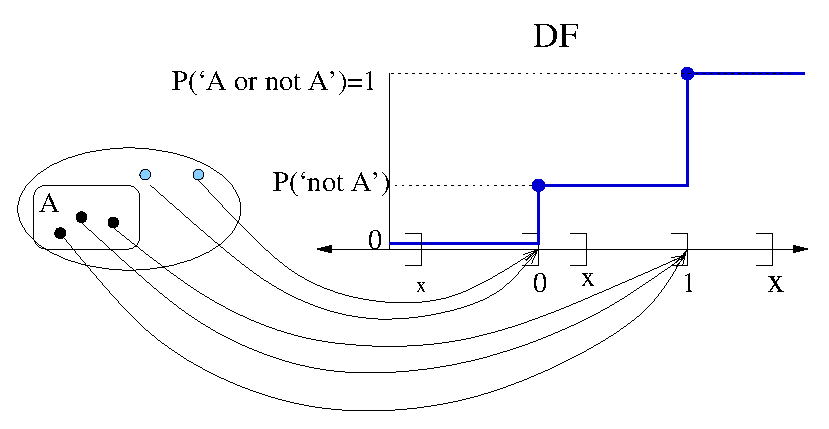
\includegraphics{figures/RVIndic}}
\end{figure}
\begin{classwork}[Indicator function is a random variable]
Let us convince ourselves that $\BB{1}_A$ is really a RV.  For $\BB{1}_A$ to be a RV, we need to verify that 
for any real number $x \in \Rz$, the inverse image $\BB{1}_A^{[-1]}( \ (- \infty, x] \ )$ is an event, ie :
\[
\BB{1}_A^{[-1]}( \ (- \infty, x] \ ) := \{\omega: \BB{1}_A(\omega) \leq x\} \in \C{F} \ .
\] 
All we can assume about the collection of events $\C{F}$ is that it contains the event $A$ and that it is a sigma algebra.  A careful look at the \hyperref[F:RVIndic]{Figure \ref*{F:RVIndic}} yields:
\begin{equation}
\BB{1}_A^{[-1]}( \ (- \infty, x] \ ) := \{\omega: \BB{1}_A(\omega) \leq x\} =
\begin{cases}
\emptyset & \text{if} \quad x < 0 \notag \\
A^c       & \text{if} \quad 0 \leq x < 1 \notag \\
A \cup A^c  = \Omega   & \text{if} \quad 1 \leq x  \notag 
\end{cases}
\end{equation}
Thus, $\BB{1}_A^{[-1]}( \ (- \infty, x] \ )$ is one of the following three sets that belong to $\C{F}$; (1) $\emptyset$, (2) $A^c$ and (3) $\Omega$ depending on the value taken by $x$ relative to the interval $[0,1]$.  We have proved that $\BB{1}_A$ is indeed a RV.
\end{classwork}
Some useful properties of the Indicator Function are:
\[
\BB{1}_{A^c} = 1 - \BB{1}_A, \qquad \BB{1}_{A \cap B} = \BB{1}_A \BB{1}_B, \qquad \BB{1}_{A \cup B} = \BB{1}_A + \BB{1}_B - \BB{1}_A \BB{1}_B
\]
We slightly abuse notation when $A$ is a single element set by ignoring the curly braces.
\begin{figure}[htpb]
\caption{A RV $X$ from a sample space $\Omega$ with $8$ elements to $\Rz$ and its DF $F$ \label{F:RVABC}}
\centering   \makebox{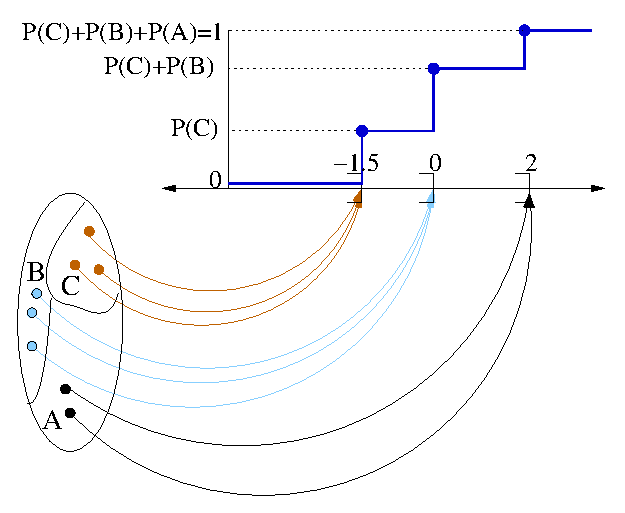
\includegraphics{figures/RV}}
\end{figure}
\begin{classwork}[A random variable with three values and eight sample points]
Consider the RV $X$ of \hyperref[F:RVABC]{Figure \ref*{F:RVABC}}.  Let the events $A = \{\omega_1, \omega_2\}$, $B = \{\omega_3, \omega_4, \omega_5\}$ and $C = \{\omega_6, \omega_7,\omega_8 \}$.  Define the RV $X$ formally.  What sets should $\C{F}$ minimally include?  What do you need to do to make sure that $\C{F}$ is a sigma algebra?
\vspace{4cm}
\end{classwork}

\section{An Elementary Discrete Random Variable}\label{S:ElemDiscRV}

When a RV takes at most countably many values from a discrete set $\Dz \subset \Rz$, we call it a {\bf discrete} RV.  Often, $\Dz$ is the set of integers $\Zz$.
\begin{definition}[probability mass function (PMF)]
Let $X$ be a discrete RV over a probability triple $(\Omega, \C{F},P)$.  We define the {\bf probability mass function} (PMF) $f$ of $X$ to be the function $f : \Dz \rightarrow [0,1]$ defined as follows:
\[
f(x) := \p(X=x) = \p( \ \{\omega: X(\omega) = x\} \ ), \qquad \text{where $x \in \Dz$.} 
\]
\end{definition}
The DF $F$ and PMF $f$ for a discrete RV $X$ satisfy the following:
\begin{enumerate}
\item  For any $x \in \Rz$,
\[
\p(X \leq x) = F(x) = \sum_{\Dz \ni y \leq x} f(y) := 
\sum_{y \ \in \  \Dz \cap (-\infty, x] } f(y) \ .
\]
\item For any $a,b \in \Dz$ with $a<b$,
\[
\p(a < X \leq b) = F(b) - F(a) = \sum_{y \ \in \  \Dz \cap (a, b] } f(y) \ .
\]
In particular, when $\Dz=\Zz$ and $a=b-1$,
\[
\p(b-1 < X \leq b) = F(b) - F(b-1) = f(b) = \p( \ \{ \omega : X(\omega) = b\} \ ) \ .
\]
\item And of course
\[
% \lim_{x \rightarrow \infty} F_X(x) = 1
\sum_{x \in \Dz} f(x) = 1
\]
\end{enumerate}

The Indicator Function $\BB{1}_A$ of the event that `$A$ occurs' for the $\theta$-specific experiment $\E{E}$ over some probability triple $(\Omega,\C{F},\p_{\theta})$, with $A \in \C{F}$, is the $\bernoulli(\theta)$ RV.  The parameter $\theta$ denotes the probability that `$A$ occurs' (see \hyperref[F:RVt1T]{Figure \ref*{F:RVt1T}} when $A$ is the event that `{\tt H} occurs').  This is our first example of a discrete RV.

\begin{model}[$\bernoulli(\theta)$]
Given a parameter $\theta \in [0,1]$, the probability mass function (PMF) for the $\bernoulli(\theta)$ RV $X$ is:
\begin{equation}\label{E:Bernoullipdf}
f(x;\theta)= \theta^x (1-\theta)^{1-x} \BB{1}_{\{0,1\}}(x) =
\begin{cases}
\theta & \text{if $x=1$,}\\
1-\theta & \text{if $x=0$,}\\
0 & \text{otherwise}
\end{cases}
\end{equation}
and its DF is:
\begin{equation}
F(x;\theta) =
\begin{cases}
1 & \text{if $1 \leq x$,}\\
1-\theta & \text{if $0 \leq x < 1$,}\\
0 & \text{otherwise}
\end{cases}
\end{equation}
We emphasise the dependence of the probabilities on the parameter $\theta$ by specifying it following the semicolon in the argument for $f$ and $F$ and by subscripting the probabilities, i.e.~$\p_{\theta}(X=1)=\theta$ and $\p_{\theta}(X=0)=1-\theta$.
\end{model}
\begin{figure}[htpb]
\caption{The Indicator Function $\BB{1}_{ \ {\tt H} \ }$ of the event `Heads occurs', for the experiment `Toss 1 times,' $\E{E}_{\theta}^{1}$, as the RV $X$ from the sample space $\Omega = \{ {\tt H}, {\tt T}\}$ to $\Rz$ and its DF $F$.  The probability that `Heads occurs' and that `Tails occurs' are $f(1;\theta)=\p_{\theta}(X=1) = \p_{\theta}({\tt H})=\theta$ and $f(0;\theta)=\p_{\theta}(X=0)=\p_{\theta}({\tt T})=1-\theta$, respectively.\label{F:RVt1T}}
\centering   \makebox{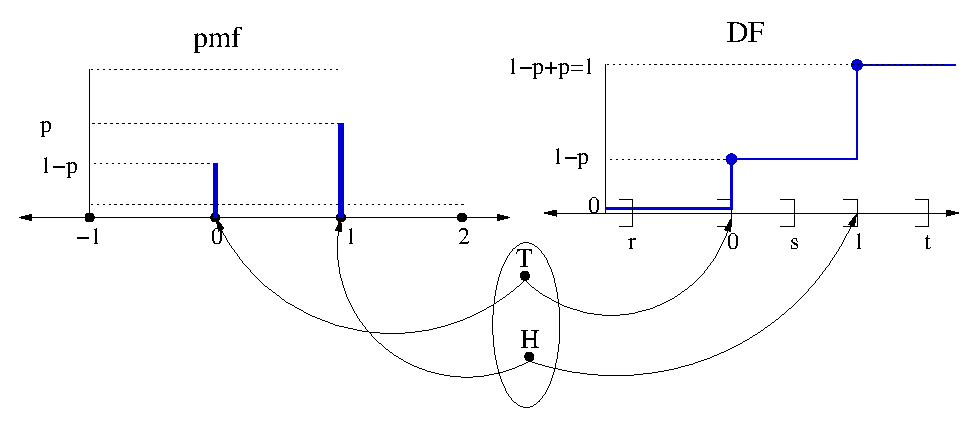
\includegraphics[width=6.5in]{figures/RVToss1}}
\end{figure}

\section{An Elementary Continuous Random Variable}\label{S:ElemContRV}

When a RV takes values in the continuum we call it a {\bf continuous} RV.  An example of such a RV is the vertical position (in micro meters) since the original release of a pollen grain on water.  Another example of a continuous RV is the volume of water (in cubic meters) that fell on the southern Alps last year.  
\begin{definition}[probability density function (PDF)]
A RV $X$ is said to be `continuous' if there exists a piecewise-continuous function $f$, called the probability density function (PDF) of $X$, such that for any $a, b \in \Rz$ with $a < b$,
\[
\p(a < X \leq b) = F(b)-F(a) = \int_a^b f(x) \ dx \ .
\]
\end{definition}
The following hold for a continuous RV $X$ with PDF $f$:
\begin{enumerate}
\item For any $x \in \Rz$, $\p(X=x)=0$.
\item Consequentially, for any $a,b \in \Rz$ with $a \leq b$,
\[
\p(a < X < b ) = \p(a < X \leq b) = \p(a \leq X \leq b) = \p(a \leq X < b) \ .
\]
\item By the fundamental theorem of calculus, except possibly at finitely many points (where the continuous pieces come together in the piecewise-continuous $f$):
\[
f(x) = \frac{d}{dx} F(x)
\]
\item And of course $f$ must satisfy:
\[
\int_{-\infty}^{\infty} f(x) \ dx = \p(-\infty < X < \infty) = 1 \ .
\] 
\end{enumerate}

An elementary and fundamental example of a continuous RV is the $\uniform(0,1)$ RV of \hyperref[M:Uniform01]{Model \ref*{M:Uniform01}}.  It forms the foundation for random variate generation and simulation.  In fact, it is appropriate to call this the fundamental model since every other experiment can be obtained from this one.

\begin{model}[The Fundamental Model]\label{M:Uniform01}
The probability density function (PDF) of the fundamental model or the $\uniform(0,1)$ RV is
\begin{equation}\label{E:Uniform01pdf}
f(x) = \BB{1}_{[0,1]}(x) = 
\begin{cases}
1 & \text{if $0 \leq x \leq 1$,}\\
0 & \text{otherwise}
\end{cases}
\end{equation}
and its distribution function (DF) or cumulative distribution function (CDF) is:
\begin{equation}\label{E:Uniform01DF}
F(x) := \int_{- \infty}^x f(y) \ dy =
\begin{cases}
0 & \text{if $x < 0$,} \\
x & \text{if $0 \leq x \leq 1$,}\\
1 & \text{if $x > 1$} 
\end{cases}
\end{equation}
Note that the DF is the identity map in $[0,1]$.  The PDF and DF are depicted in \hyperref[F:unif01]{Figure~\ref*{F:unif01}}.
\begin{figure}[htpb]
\caption{A plot of the PDF and DF or CDF of the $\uniform(0,1)$ continuous RV $X$.\label{F:unif01}}
\centering   \makebox{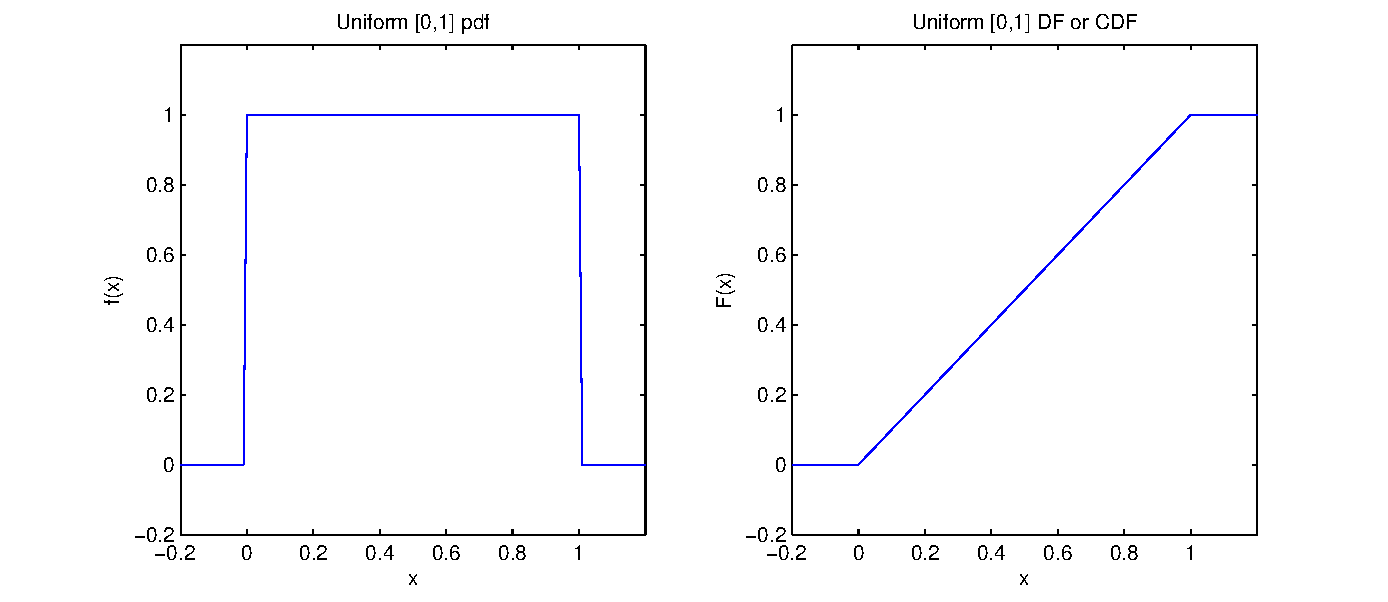
\includegraphics[width=6.5in]{figures/Unif01pdfcdf}}
\end{figure}
\end{model}

\remove{
\begin{labwork}[PDF of $\uniform(0,1)$ RV]\label{LW:Unif01Pdf}
Let us encode the PDF of $\uniform(0,1)$ as an M-file in {\sc Matlab}.  Notice that the PDF function assigns $1$ to every value of $x \in [0,1]$ and $0$ to every value of $x \notin [0,1]$.  So, the problem mostly boils down to finding the entries inside and outside the range.  We can use {\sc Matlab}'s built-in {\tt find} function for this purpose.  We give an example to illustrate the syntax of {\tt find}.
\begin{VrbM}
>> Xs=[0.2511    1.6160    0.4733    -5.3517    0.8308    0.5853    2.5497] % an array Xs with real values 
Xs =    0.2511    1.6160    0.4733   -5.3517    0.8308    0.5853    2.5497
\end{VrbM}
We can obtain the indices of {\tt Xs} whose values are $\geq 0$, i.e.~$\{i: {\tt Xs}(i) \geq 0 \}$ and the indices of {\tt Xs} whose values are $\leq 1$, i.e.~$\{i: {\tt Xs}(i) \leq 1 \}$ as follows:
\begin{VrbM}
>> find(Xs >= 0)
ans =     1     2     3     5     6     7
>> find(Xs <= 1)
ans =     1     3     4     5     6
\end{VrbM}
The intersection of the two sets of indices, i.e.~$\{i: {\tt Xs}(i) \geq 0 \ \text{ and } \  {\tt Xs}(i) \leq 1 \} = \{i: 0 \leq {\tt Xs}(i) \leq 1 \}$ can be obtained by {\tt \&}, the Boolean and, as follows:
\begin{VrbM}
>> find(Xs >= 0 & Xs <= 1)
ans =     1     3     5     6
\end{VrbM}
Finally, we know which indices of the {\tt Xs} array should have the PDF value of $1$.  The remaining indices of {\tt Xs} should therefore have the PDF value of $0$.  Let us declare an array called {\tt Pdf} for the PDF values corresponding to the {\tt Xs}.  We can initialise this array with zeros using the {\tt zeros} function and make it of the same size as {\tt Xs} as follows:
\begin{VrbM}
>> size(Xs)
ans =     1     7
>> Pdf = zeros(1,7)
Pdf =     0     0     0     0     0     0     0
\end{VrbM}
Now, we can set the indices $1,3,5,6$ (returned by {\tt find(Xs >= 0 \& Xs <= 1)}) of {\tt Pdf} array to 1.
\begin{VrbM}
>> Pdf([1     3     5     6])=1
Pdf =     1     0     1     0     1     1     0
\end{VrbM}
We can modularise this process for an arbitrary input array {\tt x} via a function in the following M-file.
\VrbMf[label=Unif01Pdf.m]{scripts/Unif01Pdf.m} 
Let us call the function we wrote called {\tt Unif01Pdf} next.
\begin{VrbM}
>> help Unif01Pdf
  Unif01Pdf(x) returns the PDF of Uniform(0,1) RV X
  the input x can be an array
>> Xs
Xs =    0.2511    1.6160    0.4733   -5.3517    0.8308    0.5853    2.5497
>> Unif01Pdf(Xs)
ans =     1     0     1     0     1     1     0
\end{VrbM}
\end{labwork}

\begin{labwork}[CDF of $\uniform(0,1)$ RV]\label{LW:Unif01Cdf}
Understand each step in the function {\tt Unif01Cdf}:
\VrbMf[label=Unif01Cdf.m]{scripts/Unif01Cdf.m} 
When we type in {\tt help Unif01Cdf}, {\tt Xs} and {\tt Unif01Cdf(Xs)} we can confirm that the {\tt Unif01Cdf} function is correctly reporting the CDF values of the input array {\tt Xs}.
\begin{VrbM}
>> help Unif01Cdf
  Unif01Cdf(x) returns the CDF of Uniform(0,1) RV X
  the input x can be an array 
>> Xs
Xs =    0.2511    1.6160    0.4733   -5.3517    0.8308    0.5853    2.5497
>> Unif01Cdf(Xs)
ans =    0.2511    1.0000    0.4733         0    0.8308    0.5853    1.0000
\end{VrbM}
\end{labwork}

\begin{labwork}[Plot of the PDF and the CDF for the $\uniform(0,1)$ RV]\label{LW:PlotUnif01PdfCdf}
Generate the plot of the PDF and the CDF for the $\uniform(0,1)$ RV $X$ by following the commands below.  Go through every step and understand each command when you reproduce the plot.
\VrbMf[label=plotunif.m]{scripts/plotunif.m} 
The plot was saved as an encapsulated postscript file from the File menu of the Figure window and is displayed in \hyperref[F:unif01]{Figure~\ref*{F:unif01}}.
 \end{labwork}
}

{\bf **tossing a fair coin infinitely often and the fundamental model}

%TODO\input{figures/UnifsInUnif.tex}

--- The fundamental model is equivalent to infinite tosses of a fair coin (see using binary expansion of any $x \in (0,1)$)

--- The fundamental model has infinitely many copies of itself within it!


{\bf **universality of the fundamental model}

--- one can obtain any other random object from the fundamental model!

\section{Transformations of random variables}\label{S:TransformationsOFRvs}

Suppose we know the distribution of a random variable $X$.  How do we find the distribution of a transformation of $X$, say $g(X)$?
Before we answer this question let us ask a motivational question.  Why are we interested in functions of random variables?

\begin{example}
Consider a simple financial example where an individual sells $X$ items per day, the profit per item is $\$ 5$ and the overhead costs are $\$ 500$ per day.  The original random variable is $X$, but the random variable $Y$ which gives the daily profit is of more interest, where
\[
Y = 5X - 500 \enspace . 
\]
\end{example}

\begin{example}
In a cell-phone system a mobile signal may have a signal-to-noise-ratio of $X$, but engineers prefer to express such ratios in decibels, i.e.,
\[
Y = 10 \log_{10}(X) \enspace .
\]
\end{example}

Hence in a great many situations we are more interested in functions of random variables. 
Let us return to our original question of determining the distribution of a transformation or function of $X$.  
First note that this transformation of $X$ is itself another random variable, say $Y = g(X)$, 
where $g$ is a function from a subset $\mathbb{X}$ of $\mathbb{R}$ to a subset $\mathbb{Y}$ of $\mathbb{R}$, 
i.e., $g: \mathbb{X} \to \mathbb{Y}$, $\mathbb{X} \subset \mathbb{R}$ and $\mathbb{Y} \subset \mathbb{R}$.

The {\bf inverse image} of a set $A$ is the set of all real numbers in $\mathbb{X}$ whose image is in $A$, i.e.,
\[
g^{[-1]}(A) = \{x \in \mathbb{X} : g(x) \in A \} \enspace .
\] 
In other words,
\[
x \in g^{[-1]}(A) \ \text{if and only if} \ g(x) \in A \enspace .
\]
For example,
\begin{itemize}
\item if $g(x)=2x$ then $g^{[-1]}([4,6])=[2,3]$
\item if $g(x)=2x+1$ then $g^{[-1]}([5,7])=[2,3]$
\item if $g(x)=x^3$ then $g^{[-1]}([1,8])=[1,2]$
\item if $g(x)=x^2$ then $g^{[-1]}([1,4])=[-2,-1] \cup [1,2]$
\item if $g(x)=\sin(x)$ then $g^{[-1]}([-1,1])=\mathbb{R}$
\item if ... %Raaz add other examples of the transformations done in the sequel here
\end{itemize}
For the singleton set $A = \{y\}$, we write $g^{[-1]}(y)$ instead of $g^{[-1]}(\{y\})$.  
For example,
\begin{itemize}
\item if $g(x)=2x$ then $g^{[-1]}(4)=\{2\}$
\item if $g(x)=2x+1$ then $g^{[-1]}(7)=\{3\}$
\item if $g(x)=x^3$ then $g^{[-1]}(8)=\{2\}$
\item if $g(x)=x^2$ then $g^{[-1]}(4)=\{-2,2\}$
\item if $g(x)=\sin(x)$ then $g^{[-1]}(0)=\{k \pi: k \in \mathbb{Z}\} = \{\ldots, -3 \pi, -2 \pi, -\pi,0,\pi, 2\pi,3\pi, \ldots\}$
\item if ... %Raaz add other examples of the transformations done in the sequel here
\end{itemize}
If $g:\mathbb{X}\to\mathbb{Y}$ is one-to-one (injective) and onto (surjective), then the inverse image of a singleton set is itself a singleton set.  
Thus, the inverse image of such a function $g$ becomes itself a function and is called the {\bf inverse function}.
One can find the inverse function, if it exists by the following steps:
\begin{itemize}
\item[{\sf Step 1;}] write $y=g(x)$
\item[{\sf Step 2;}] solve for $x$ in terms of $y$
\item[{\sf Step 3;}] set $g^{-1}(y)$ to be this solution
\end{itemize}
We write $g^{-1}$ whenever the inverse image $g^{[-1]}$ exists as an inverse function of $g$.  
Thus, the inverse function $g^{-1}$ is a specific type of inverse image $g^{[-1]}$.  
For example,
\begin{itemize}
\item if $g(x)=2x$ then $g:\mathbb{R} \to \mathbb{R}$ is injective and surjective and therefore its inverse function is:\\
{\sf Step 1;} $y=2x$, {\sf Step 2;} $x=\frac{y}{2}$, {\sf Step 3;} $g^{-1}(y)=\frac{y}{2}$
\item if $g(x)=2x+1$ then $g:\mathbb{R} \to \mathbb{R}$ is injective and surjective and therefore its inverse function is:\\
{\sf Step 1;} $y=2x+1$, {\sf Step 2;} $x=\frac{y-1}{2}$, {\sf Step 3;} $g^{-1}(y)=\frac{y-1}{2}$
\item if $g(x)=x^3$ then $g:\mathbb{R} \to \mathbb{R}$ is injective and surjective and therefore its inverse function is:\\
{\sf Step 1;} $y=x^3$, {\sf Step 2;} $x={y}^{\frac{1}{3}}$, {\sf Step 3;} $g^{-1}(y)={y}^{\frac{1}{3}}$
\end{itemize}
However, you need to be careful by limiting the domain to obtain the inverse function for the following examples:
\begin{itemize}
\item if $g(x)=x^2$ and domain of $g$ is $[0,+\infty)$ then its inverse function is $g^{-1}(y)=\sqrt{y}$, 
i.e., if $g(x)=x^2 : [0,+\infty) \to [0,+\infty)$ then the inverse image $g^{[-1]}(y)$ for $y \in [0,+\infty)$ is given by the inverse function $g^{-1}(y)=\sqrt{y} : [0,+\infty) \to [0,+\infty)$.
\item if $g(x)=x^2$ and domain of $g$ is $(-\infty,0]$ then its inverse function is $g^{-1}(y)=-\sqrt{y}$, 
i.e., if $g(x)=x^2 : (-\infty,0] \to [0,+\infty)$ then the inverse image $g^{[-1]}(y)$ for $y \in [0,+\infty)$ is given by the inverse function $g^{-1}(y)=-\sqrt{y} : [0,+\infty) \to (-\infty,0]$.
\item if $g(x)=\sin(x)$ and domain of $g$ is $[0,\frac{\pi}{2}]$ then its inverse function $g^{-1}(y)=\arcsin(y)$, i.e., if $g(x)=\sin(x) : [0,\frac{\pi}{2}] \to [0,1]$ then the inverse image $g^{[-1]}(y)$ for $y \in [0,1]$ is given by the inverse function $g^{-1}(y)=\arcsin(y) : [0,1] \to [0, \frac{\pi}{2}]$.
\item if $g(x)=\sin(x)$ and domain of $g$ is $[-\frac{\pi}{2},\frac{\pi}{2}]$ then its inverse function $g^{-1}(y)=\arcsin(y)$, i.e., if $g(x)=\sin(x) : [-\frac{\pi}{2},\frac{\pi}{2}] \to [-1,1]$ then the inverse image $g^{[-1]}(y)$ for $y \in [-1,1]$ is given by the inverse function $g^{-1}(y)=\arcsin(y) : [-1,1] \to [-\frac{\pi}{2},\frac{\pi}{2}]$.
\item if ... %Raaz add other examples of the transformations done in the sequel here
\end{itemize}
  
Now, let us return to our question of determining the distribution of the transformation $g(X)$.  To answer this question we must first observe that the inverse image $g^{[-1]}$ satisfies the following properties:
\begin{itemize}
\item $g^{[-1]}(\mathbb{Y}) = \mathbb{X}$
\item For any set $A$, $g^{[-1]}(A^c) = \left(g^{[-1]}(A)\right)^c$
\item For any collection of sets $\{A_1,A_2,\ldots\}$,
\[
g^{[-1]}\left( A_1 \cup A_2 \cup \cdots \right) = g^{[-1]}(A_1) \cup g^{[-1]}(A_2) \cup \cdots \enspace.
\]
\end{itemize}
Consequentially, 
\begin{equation}\label{E:ProbOfgOfX}
\boxed{P \left( g(X) \in A \right) = P \left(X \in g^{[-1]}(A) \right)}
\end{equation} 
satisfies the axioms of probability and gives the desired probability of the event $A$ from the transformation $Y=g(X)$ in terms of the probability of the event given by the inverse image of $A$ underpinned by the random variable $X$.  
It is crucial to understand this from the sample space $\Omega$ of the underlying experiment in the sense that Equation~\eqref{E:ProbOfgOfX} is just short-hand for its actual meaning:
\[
P \left( \{\omega \in \Omega: g(X(\omega)) \in A\} \right) 
= P \left( \left\{ \omega \in \Omega: X(\omega) \in g^{[-1]}(A) \right\} \right) \enspace .
\]
Because we have more than one random variable to consider, namely, $X$ and its transformation $Y=g(X)$ we will subscript the probability density or mass function and the distribution function by the random varaible itself.  For example we denote the distribution function of $X$ by $F_X(x)$ and that of $Y$ by $F_Y(y)$.

\subsection{Transformation of discrete random variables}
For a discrete random variable $X$ with probability mass function $f_X$ we can obtain the probability mass function $f_Y$ of $Y=g(X)$ using Equation~\eqref{E:ProbOfgOfX} as follows:
\begin{eqnarray*}
f_Y(y) 
&=& P(Y =y) = P(Y \in \{y\}) \\
&=& P \left( g(X) \in \{y\} \right) = P \left(X \in g^{[-1]}(\{y\}) \right)\\
&=& P \left(X \in g^{[-1]}(y) \right) = \sum_{x \in g^{[-1]}(y)} f_X(x) = \sum_{x \in \{x: g(x)=y\}} f_X(x) \enspace .
\end{eqnarray*}
This gives the formula:
\begin{equation}\label{E:PMFOfgOfX}
\boxed{
f_Y(y) = P(Y =y) = \sum_{x \in g^{[-1]}(y)} f_X(x) = \sum_{x \in \{x: g(x)=y\}} f_X(x) \enspace .
}
\end{equation}

\begin{example}\label{EXMP:Discrete1to1TransYis2X}
Let $X$ be the discrete random variable with probability mass function $f_X$ as tabulated below:\\
\begin{center}
\begin{tabular}{r|rrr}
$x$ & -1 & 0 & 1\\ \hline
 &  &  & \\ 
$f_X(x)=P(X=x)$ & $\frac{1}{4}$ & $\frac{1}{2}$ & $\frac{1}{4}$
\end{tabular}
\end{center}
If $Y=2X$ then the transformation $g(X)=2X$ has inverse image $g^{[-1]}(y)=\{y/2\}$.  
Then, by Equation~\eqref{E:PMFOfgOfX} the probability mass function of $Y$ is expressed in terms of the known probabilities of $X$ as:\\ 
$$f_Y(y)=P(Y=y)= \sum_{x \in g^{[-1]}(y)} f_X(x)  = \sum_{x \in \{y/2\}} f_X(x) = f_X(y/2) \enspace ,$$
and tabulated below:\\
\begin{center}
\begin{tabular}{r|rrr}
$y$ & -2 & 0 & 2\\ \hline
 &  &  & \\ 
$f_Y(y)$ & $\frac{1}{4}$ & $\frac{1}{2}$ & $\frac{1}{4}$
\end{tabular}
\end{center}
\end{example}

\begin{example}\label{EXMP:Discrete1to1TransYis2Xplus1}
If $X$ is the random variable in the previous Example then what is the probability mass function of $Y=2X+1$?
Once again,
$$f_Y(y)=P(Y=y)= \sum_{x \in g^{[-1]}(y)} f_X(x)  = \sum_{x \in \{(y-1)/2\}} f_X(x) = f_X((y-1)/2) \enspace ,$$
and tabulated below:\\
\begin{center}
\begin{tabular}{r|rrr}
$y$ & -1 & 1 & 3\\ \hline
 &  &  & \\ 
$f_Y(y)$ & $\frac{1}{4}$ & $\frac{1}{2}$ & $\frac{1}{4}$
\end{tabular}
\end{center}
\end{example}

In fact, obtaining the probability of a one-to-one transformation of a discrete random variable as in Examples~\ref{EXMP:Discrete1to1TransYis2X} and \ref{EXMP:Discrete1to1TransYis2Xplus1} is merely a matter of looking up the probability at the image of the inverse function.  This is because there is only one term in the sum that appears in Equation~\eqref{E:PMFOfgOfX}.  When the transformation is not one-to-one the number of terms in the sum can be more than one as shown in the next Example.

\begin{example}
Reconsider the random variable $X$ of the last two Examples and let $Y=X^2$.  
Recall that $g(x)=x^2$ does not have an inverse function unless the domain is restricted to the positive or the negative parts of the real line.  
Since our random variable $X$ takes values on both sides of the real line, namely $\{-1,0,1\}$, let us note that the transformation $g(X)=X^2$ is no longer a one-to-one function.  
Then, by Equation~\eqref{E:PMFOfgOfX} the probability mass function of $Y$ is expressed in terms of the known probabilities of $X$ as:\\ 
\[
f_Y(y)=P(Y=y)= \sum_{x \in g^{[-1]}(y)} f_X(x)  = \sum_{\{x:g(x)=y\}} f_X(x) = \sum_{\{x:x^2=y\}} f_X(x) \enspace ,
\]
computed for each $y \in \{0,1\}$ as follows:
\begin{eqnarray*}
f_Y(0) &=& \sum_{\{x:x^2=0\}} f_X(x) = f_X(0)=\frac{1}{2} \enspace ,\\
f_Y(1) &=& \sum_{\{x:x^2=1\}} f_X(x) = f_X(-1)+f_X(1)=\frac{1}{4}+\frac{1}{4}=\frac{1}{2} \enspace ,
\end{eqnarray*}
and finally tabulated below:\\
\begin{center}
\begin{tabular}{r|ccc}
$y$ & 0 & & 1\\ \hline
 &  &  & \\ 
$f_Y(y)$ & $\frac{1}{2}$ & \quad & $\frac{1}{2}$
\end{tabular}\enspace .
\end{center}
\end{example}

\subsection{Transformation of continuous random variables}
Suppose we know $F_X$ and/or $f_X$ of a continuous random variable $X$.  
Let $Y=g(X)$ be a transformation of $X$.  
Our objective is to obtain $F_Y$ and/or $f_Y$ of $Y$ from $F_X$ and/or $f_X$.  
%We will look at two techniques in Sections~\ref{S:DirectMethod} and \ref{S:f_YDirectlyFromf_X} to achieve our objective.

\subsubsection{One-to-one transformations}\label{S:f_YDirectlyFromf_X}
The easiest case for transformations of continuous random variables is when $g$ is {\bf one-to-one and monotone}.  
\begin{itemize}
\item{
First, let us consider the case when $g$ is {\bf monotone and increasing} on the range of the random variable $X$.  
In this case $g^{-1}$ is also an increasing function and we can obtain the distribution function of $Y=g(X)$ in terms of the distribution function of $X$ as   
\[
F_Y(y) =P \left(Y \leq y \right)=P \left(g(X) \leq y \right) = P \left(X \leq g^{-1}(y) \right) = F_X(g^{-1}(y)) \enspace .
\]
Now, let us use a form of chainrule to compute the density of $Y$ as follows:
\[
f_Y(y) 
= \frac{d}{dy} F_Y(y)
= \frac{d}{dy} F_X \left(g^{-1}(y) \right)
= f_X \left( g^{-1}(y) \right) \frac{d}{dy} \left(g^{-1}(y) \right) \enspace . 
\]
}
\item{
Second, let us consider the case when $g$ is {\bf monotone and decreasing} on the range of the random variable $X$.  
In this case $g^{-1}$ is also a decreasing function and we can obtain the distribution function of $Y=g(X)$ in terms of the distribution function of $X$ as   
\[
F_Y(y) =P \left(Y \leq y \right)=P \left(g(X) \leq y \right) = P \left(X \geq g^{-1}(y) \right) = 1- F_X(g^{-1}(y)) \enspace ,
\]
and the density of $Y$ as 
\[
f_Y(y) 
= \frac{d}{dy} F_Y(y)
= \frac{d}{dy} \left(1-F_X \left(g^{-1}(y) \right) \right)
= -f_X \left( g^{-1}(y) \right) \frac{d}{dy} \left(g^{-1}(y) \right) \enspace . 
\]
For a monotonic and decreasing $g$, its inverse function $g^{-1}$ is also decreasing and consequently the density $f_Y$ is indeed positive because $\frac{d}{dy} \left(g^{-1}(y) \right)$ is negative.  
}
\end{itemize}
We can combine the above two cases and obtain the following 
{\bf change of variable formula} for the probability density of $Y=g(X)$ when $g$ is one-to-one and monotone on the range of $X$.
\begin{equation}\label{E:f_YFromf_X_Under_one-to-one-g}
\boxed{
f_Y(y) = f_X \left( g^{-1}(y) \right) \left\vert \frac{d}{dy} g^{-1}(y) \right\vert \enspace .}
\end{equation}

The steps involved in finding the density of $Y=g(X)$ for a one-to-one and monotone $g$ are:
\begin{enumerate}
\item Write $y=g(x)$ for $x$ in range of $x$ and check that $g(x)$ is monotone over the required range to apply the change of variable formula. 
\item Write $x=g^{-1}(y)$ for $y$ in range of $y$.
\item Obtain $\left\vert \frac{d}{dy} g^{-1}(y) \right\vert$ for $y$ in range of $y$.
\item Finally, from Equation~\eqref{E:f_YFromf_X_Under_one-to-one-g} get $f_Y(y) = f_X \left( g^{-1}(y) \right) \left\vert \frac{d}{dy} g^{-1}(y) \right\vert$ for $y$ in range of $y$. 
\end{enumerate}

Let us use these four steps to obtain the density of monotone transformations of continuous random variables.

\begin{example}
Let $X$ be $\uniform(0,1)$ random variable and let $Y=g(X)=1-X$.  
We are interested in the density of the tranformed random variable $Y$. Let us follow the four steps and use the change of variable formula to obtain $f_Y$ from $f_X$ and $g$.
\begin{enumerate}
\item $y=g(x)=1-x$ is a monotone decreasing function over $0 \leq x \leq 1$, the range of $X$.  
So, we can apply the change of variable formula. 
\item $x=g^{-1}(y)=1-y$ is a monotone decreasing function over $1-0 \geq 1-x \geq 1-1$, i.e., $0 \leq y \leq 1$.  
\item For $0 \leq y \leq 1$,
\[
 \left\vert \frac{d}{dy} g^{-1}(y) \right\vert 
= \left\vert \frac{d}{dy} \left( 1-y \right) \right\vert 
= \left\vert -1 \right\vert = 1 \enspace .
\]
\item we can use Equation~\eqref{E:f_YFromf_X_Under_one-to-one-g} to find the density of $Y$ as follows:
\[
f_Y(y) = f_X \left( g^{-1}(y) \right) \left\vert \frac{d}{dy} g^{-1}(y) \right\vert 
= f_X \left( 1-y \right)  \, 1
= 1 \enspace ,
\]
for $0 \leq y \leq 1$
\end{enumerate}
Thus, we have shown that if $X$ is a $\uniform(0,1)$ random variable then $Y=1-X$ is also a $\uniform(0,1)$ random variable.
\end{example}

\begin{example}
Let $X$ be a $\uniform(0,1)$ random variable and let $Y=g(X)=-\log(X)$.  
We are interested in the density of the tranformed random variable $Y$.  
Once again, since $g$ is a one-to-one monotone function let us follow the four steps and use the change of variable formula to obtain $f_Y$ from $f_X$ and $g$.
\begin{enumerate}
\item $y=g(x)=-\log(x)$ is a monotone decreasing function over $0 < x < 1$, the range of $X$.  
So, we can apply the change of variable formula. 
\item $x=g^{-1}(y)=\exp(-y)$ is a monotone decreasing function over %$-\log(0) > -\log(x) > -\log(1)$, i.e., %Ben does not like -\log(0)=-\infty because -\log(0) is said to be undefined to these students -- raaz expected -\log(0) = \lim_{x \to 0^+} \log(x) = -\infty is reasonable to assume here.
$0 < y < \infty$.  
\item For $0 < y < \infty$,
\[
 \left\vert \frac{d}{dy} g^{-1}(y) \right\vert 
= \left\vert \frac{d}{dy} \left( \exp(-y) \right) \right\vert 
= \left\vert -\exp(-y) \right\vert = \exp(-y) \enspace .
\]
\item We can use Equation~\eqref{E:f_YFromf_X_Under_one-to-one-g} to find the density of $Y$ as follows:
\[
f_Y(y) = f_X \left( g^{-1}(y) \right) \left\vert \frac{d}{dy} g^{-1}(y) \right\vert 
= f_X \left( \exp(-y) \right)  \, \exp(-y)
= 1 \, \exp(-y) = \exp(-y) \enspace .
\]
Note that $0 < \exp(-y) < 1$ for $0 < y < \infty$.
\end{enumerate}
Thus, we have shown that if $X$ is a $\uniform(0,1)$ random variable then $Y=-\log(X)$ is an random variable with PDF $f_Y(y)=\BB{1}_{(0,\infty)}(y)\exp(-y)$. 
We can similarly show that for a parameter $\lambda>0$, if $X \sim \uniform(0,1)$ then $Y=-\lambda^{-1} \log(X)$ yields a probability model of RVs that are parameterized by $\lambda$ and extremely useful in applications. We introduce it next.
\end{example}

\begin{model}[$\exponential(\lambda)$]\label{M:exponential}
For a given $\lambda > 0$, an $\exponential(\lambda)$ RV has the following PDF $f$ and DF $F$:
\begin{eqnarray}\label{E:Exponentialpdfcdf}
f(x; \lambda) = \lambda e^{-\lambda x} \qquad &
F(x; \lambda)= 1-e^{-\lambda x}  \ .
\end{eqnarray}
This distribution is fundamental because of its property of {\bf memorylessness} and plays a fundamental role in continuous time
%Markov
processes as we will see later.
\end{model}

\remove{
We encode the PDF and DF of the $\exponential(\lambda)$ RV as \Matlab functions {\tt ExponentialPdf} and {\tt ExponentialCdf} and use them to produce \hyperref[F:plotPdfCdfExponentials]{Figure~\ref*{F:plotPdfCdfExponentials}} in \hyperref[Mf:ExponentialPdfCdf]{Labwork~\ref*{Mf:ExponentialPdfCdf}}.
}%end remove

\begin{figure}[htpb]
\caption{Density and distribution functions of $\exponential(\lambda)$ RVs, for $\lambda=1, 10, 10^{-1}$, in four different axes scales.\label{F:plotPdfCdfExponentials}}
\centering   \makebox{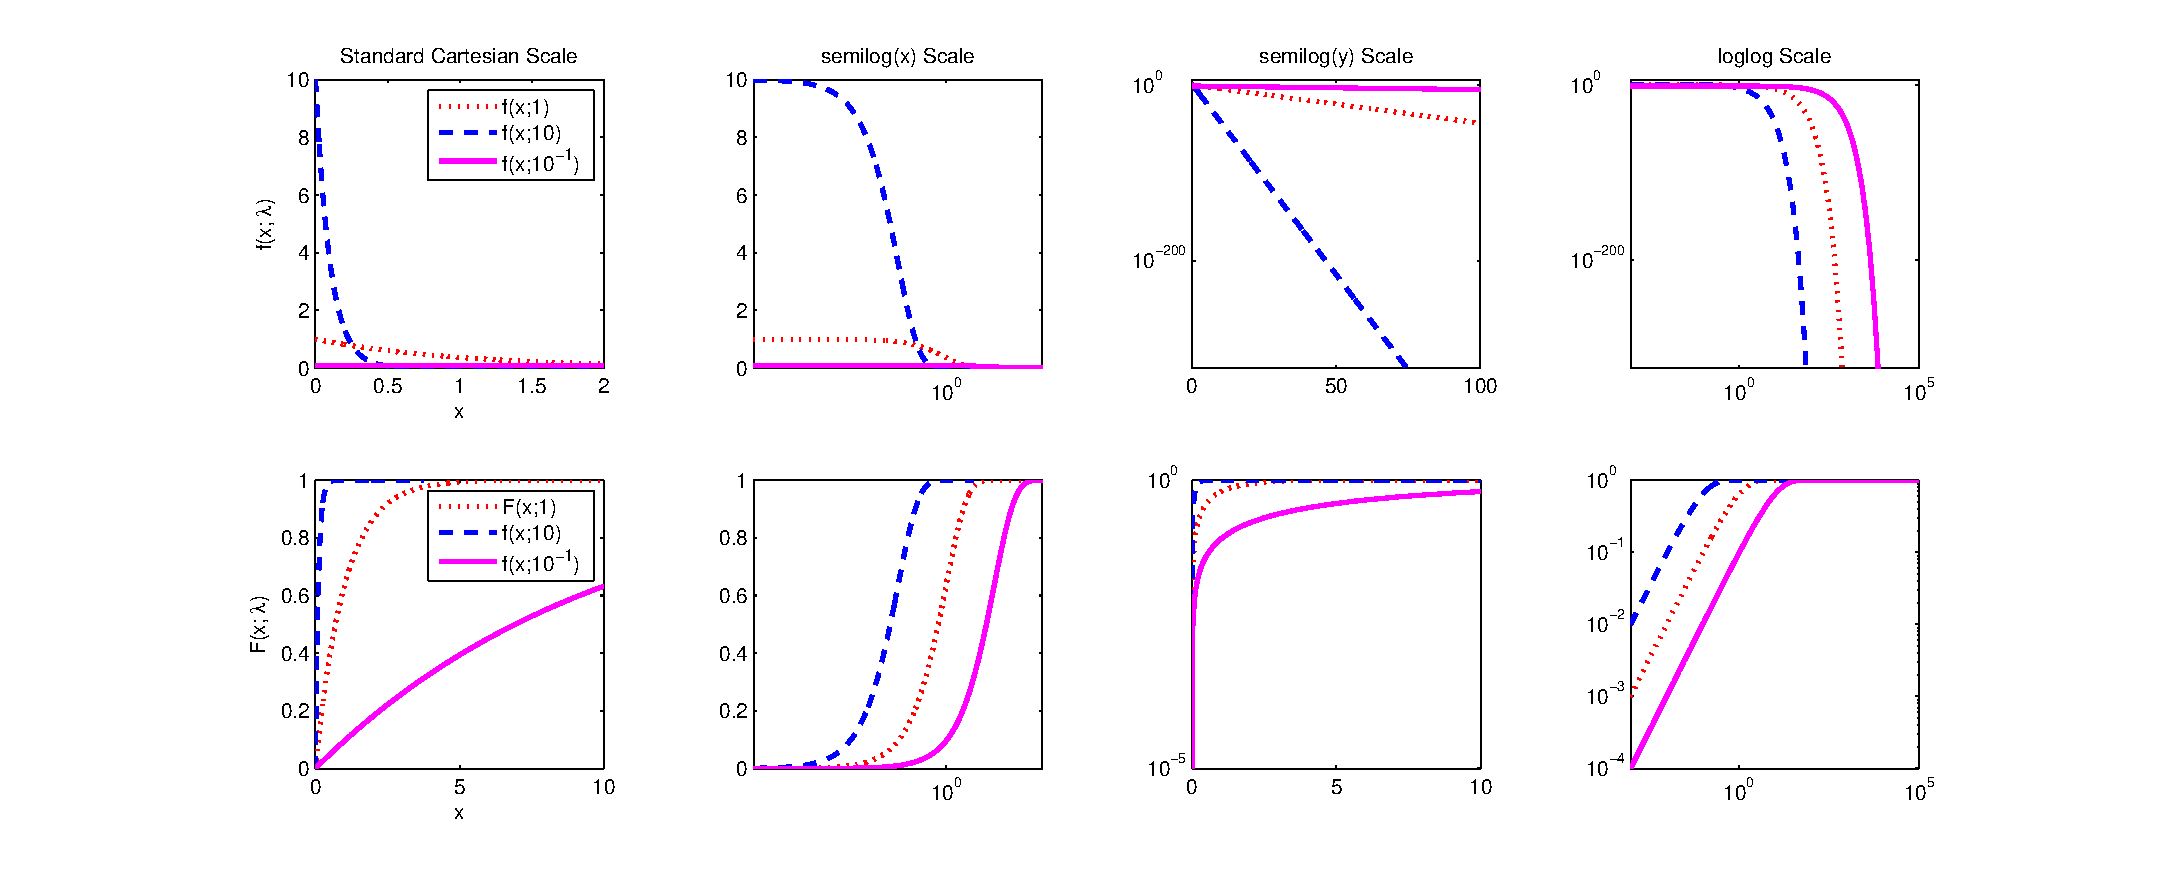
\includegraphics[width=6.5in]{figures/plotPdfCdfExponentials}}
\end{figure}


\subsubsection{Direct method}\label{S:DirectMethod}
If the transformation $g$ in $Y=g(X)$ is not necessarily one-to-one then special care is needed to obtain the distribution function or density of $Y$.  
For a continuous random variable $X$ with a known distribution function $F_X$ we can obtain the distribution function $F_Y$ of $Y=g(X)$ using Equation~\eqref{E:ProbOfgOfX} as follows:
\begin{eqnarray*}
F_Y(y)
&=& P \left(Y \leq y \right) = P \left(Y \in (-\infty, y] \right)\\
&=& P \left( g(X) \in (-\infty, y] \right) = P \left( X \in g^{[-1]}((-\infty, y]) \right) = P \left(X \in \{x: g(x) \in (-\infty,y]\}  \right) \enspace . %\\
\end{eqnarray*}
In words, the above equalities just mean that the probability that $Y \leq y$ is the probability that $X$ takes a value $x$ that satisfies $g(x) \leq y$.  
We can use this approach if it is reasonably easy to find the set $g^{[-1]}((-\infty,y]) = \{x: g(x) = (-\infty,y]\}$.% as done in Section~\ref{S:DirectMethod}.

\begin{example}
Let $X$ be any random variable with distribution function $F_X$.  Let $Y=g(X)=X^2$.  
Then we can find $F_Y$, the distribution function of $Y$ from $F_X$ as follows:
\begin{itemize}
\item {Since $Y=X^2 \geq 0$, if $y < 0$ then $F_Y(y) = P\left( X \in \{ x : x^2 < y\} \right) = P(X \in \emptyset) = 0$.}
\item {If $y \geq 0$ then
\begin{eqnarray*}
F_Y(y) = P \left(Y \leq y \right) 
&=& P \left( X^2 \leq y \right) \\
&=& P \left( -\sqrt{y} \leq X \leq \sqrt{y} \right) \\
&=& F_X(\sqrt{y}) - F_X(-\sqrt{y}) \enspace .
\end{eqnarray*}
}
\end{itemize}
By differentiation we get:
\begin{itemize}
\item {If $y<0$ then $f_Y(y)=\frac{d}{dy}(F_Y(y)) = \frac{d}{dy} 0 = 0$.}
\item {If $y \geq 0$ then
\begin{eqnarray*}
f_Y(y) 
= \frac{d}{dy}\left( F_Y(y) \right) 
&=& \frac{d}{dy}\left( F_X(\sqrt{y}) - F_X( - \sqrt{y}) \right)\\
&=& \frac{d}{dy}\left( F_X(\sqrt{y}) \right) - \frac{d}{dy}\left( F_X( - \sqrt{y}) \right)\\
&=& \frac{1}{2}y^{-\frac{1}{2}} f_X(\sqrt{y}) - \left( -\frac{1}{2}y^{-\frac{1}{2}} f_X( - \sqrt{y}) \right)\\
&=& \frac{1}{2 \sqrt{y}} \left( f_X(\sqrt{y}) + f_X( - \sqrt{y}) \right) \enspace .
\end{eqnarray*}
}
\end{itemize}
Therefore, the distribution function of $Y=X^2$ is:
\begin{equation}\label{E:F_YofX^2}
F_Y(y) = 
\begin{cases}
0 & \text{ if } y < 0 \\
F_X(\sqrt{y}) - F_X(-\sqrt{y}) & \text{ if } y \geq 0 \enspace .
\end{cases}
\end{equation}
and the probability density function of $Y=X^2$ is:
\begin{equation}\label{E:f_YofX^2}
f_Y(y) = 
\begin{cases}
0 & \text{ if } y < 0 \\
\frac{1}{2 \sqrt{y}} \left( f_X(\sqrt{y}) + f_X( - \sqrt{y}) \right) & \text{ if } y \geq 0 \enspace .
\end{cases}
\end{equation}
\end{example} 

\newpage

\section{$\Rz^m$-valued Random Variables}\label{S:RVecs}

Often, in experiments we are measuring two or more aspects simultaneously.  
For example, we may be measuring the diameters and lengths of cylindrical shafts manufactured in a plant or heights, weights and blood-sugar levels of individuals in a clinical trial.  
Thus, the underlying outcome $\omega \in \Omega$ needs to be mapped to measurements as realizations of random vectors in the real plane $\Rz^2 = (-\infty, \infty) \times (-\infty, \infty)$ or the real space $\Rz^3 = (-\infty, \infty) \times (-\infty, \infty) \times (-\infty, \infty)$:
\[
\omega \mapsto \left( X(\omega),Y(\omega) \right) : \Omega \to \Rz^2  \qquad \qquad \qquad \omega \mapsto \left( X(\omega),Y(\omega), Z(\omega) \right) : \Omega \to \Rz^3
\]
%\vspace{2cm}

More generally, we may be interested in heights, weights, blood-sugar levels, family medical history, known allergies, etc. of individuals in the clinical trial and thus need to make $m$ measurements of the outcome in $\Rz^m$ using a ``measurable mapping'' from $\Omega \to \Rz^m$.  
To deal with such multivariate measurements we need the notion of {\bf random vectors} ({\rv}s), i.e.~ordered pairs of random variables $(X,Y)$, ordered triples of random variables $(X,Y,Z)$, or more generally ordered $m$-tuples of random variables $(X_1,X_2,\ldots,X_m)$.  

\subsection{$\Rz^2$-valued Random Variables}

We first focus on understanding $(X,Y)$, a bivariate \rv~or $\Rz^2$-valued RV that is obtained from a pair of discrete or continuous RVs.  
We then generalize to $\Rz^m$-valued RVs with $m>2$ in the next section.

\begin{definition}[JDF]\label{Df:JDF}
The {\bf joint distribution function (JDF)} or {\bf joint cumulative distribution function (JCDF)}, $F_{X,Y}(x,y):\mathbb{R}^2\to [0,1]$, of the bivariate random vector $(X,Y)$ is
\begin{eqnarray}\label{E:j2DF}
F_{X,Y}(x,y)\; 
&=& \p(X\leq x \cap Y \leq y) \;= \;\p(X\leq x , Y \leq y)\notag\\
&=& P\left( \{ \omega: X(\omega) \le x, Y(\omega) \le y \} \right) \mbox{, for any } (x,y) \in \mathbb{R}^2 \enspace ,
\end{eqnarray}
where the right-hand side represents the probability that the random vector $(X,Y)$ takes on a value in 
$\{(x',y'): x' \leq x, y' \leq y\}$, the set of points in the plane that are south-west of the point $(x,y)$.
\end{definition}

The JDF $F_{X,Y}(x,y):\Rz^2\to\Rz$ satisfies the following conditions to remain a probability: 
\begin{enumerate}
\item $0 \leq F_{X,Y}(x,y) \leq 1$
\item $F_{X,Y}(x,y)$ is an non-decreasing function of both $x$ and $y$
\item $F_{X,Y}(x,y) \to 1$ as $x\to \infty$ and $y\to \infty$
\item $F_{X,Y}(x,y) \to 0$ as $x\to -\infty$ and $y\to -\infty$
\end{enumerate}

\begin{definition}[JPMF]
If $(X,Y)$ is a {\bf discrete random vector} that takes values in a discrete support set $\mathcal{S}_{X,Y} = \{(x_i,y_j): i=1,2,\ldots, \, j=1,2,\ldots\} \subset \Rz^2$ with probabilities $p_{i,j}=\p(X=x_i,Y=y_j)>0$, then its \textbf{joint probability mass function} (or JPMF) is:
\begin{equation}\label{Eq:j2DPMF}
f_{X,Y}(x_i,y_j) = \p(X=x_i,Y=y_j) %P\left(\{\omega: X(\omega) = x_i, Y(\omega)=y_j \}\right) 
=\begin{cases}
p_{i,j}&\quad \textrm{if } (x_i,y_j) \in \mathcal{S}_{X,Y}\\
0&\quad \textrm{otherwise}
\end{cases}  \enspace .
\end{equation}

Since $\p(\Omega)=1$, $\sum_{{\substack{(x_i,y_j) \in \mathcal{S}_{X,Y}}}}f_{X,Y}(x_i,y_j)=1$.
\end{definition}

From JPMF $f_{X,Y}$ we can get the values of the JDF $F_{X,Y}(x,y)$ and the probability of any event $B$ by simply taking sums,
\begin{equation}\label{Eq:2DiscretejDFFromjPMF}
\boxed{F_{X,Y}(x,y)\;=\;\sum_{x_i\leq x, y_j \leq y}f_{X,Y}(x_i,y_j) }\enspace ,
\qquad \boxed{\p(B)\;=\;\sum_{\substack{(x_i, y_j) \in B \cap \mathcal{S}_{X,Y}}}f_{X,Y}(x_i,y_j) }\enspace ,
\end{equation}

\begin{example}\label{Eg:Discrete2DPMF}
Let $(X,Y)$ be a discrete bivariate \rv with the following joint probability mass function (JPMF):
\[
f_{X,Y}(x,y) := P (X=x,Y=y)  = 
\begin{cases}
0.1 & \text{ if } (x,y)=(0,0)\\
0.3 & \text{ if } (x,y)=(0,1)\\
0.2 & \text{ if } (x,y)=(1,0)\\
0.4 & \text{ if } (x,y)=(1,1)\\
0.0 & \text{ otherwise.}
\end{cases} 
\]
\begin{center}
\makebox{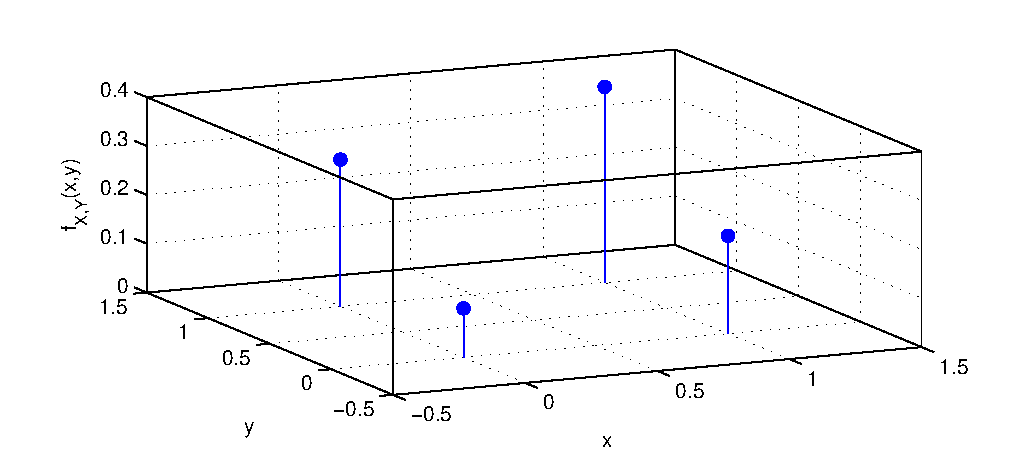
\includegraphics[width=5.0in]{figures/Discrete2DPMF}}
\end{center}
It is helpful to write down the JPMF $f_{X,Y}(x,y)$ in a tabular form:
\begin{center}
\begin{tabular}{|c|c c|}
\hline
& $Y=0$ & $Y=1$ \\ \hline
$X=0$& $0.1$ & $0.3$  \\
$X=1$& $0.2$ & $0.4$  \\ \hline
\end{tabular}
\end{center}
From the above Table we can read for instance that the joint probability $f_{X,Y}(0,0)=0.1$.

Find $\p(B)$ for the event $B=\{(0,0),(1,1)\}$, $F_{X,Y}(1/2,1/2)$, $F_{X,Y}(3/2,1/2)$, $F_{X,Y}(4,5)$ and $F_{X,Y}(-4,-1)$.

\begin{enumerate}
\item $\p(B) = \sum_{(x,y) \in \{(0,0),(1,1)\}}f_{X,Y}(x,y) = f_{X,Y}(0,0)+f_{X,Y}(1,1)=0.1+0.4$
\item $F_{X,Y}(1/2,1/2) = \sum_{\{(x,y): x\leq 1/2, y \leq 1/2\}} f_{X,Y}(x,y)=f_{X,Y}(0,0)=0.1$
\item $F_{X,Y}(3/2,1/2) = \sum_{\{(x,y): x\leq 3/2, y \leq 1/2\}} f_{X,Y}(x,y)=f_{X,Y}(0,0)+f_{X,Y}(1,0)=0.1+0.2=0.3$
\item $F_{X,Y}(4,5) = \sum_{\{(x,y): x\leq 4, y \leq 5\}} f_{X,Y}(x,y)=f_{X,Y}(0,0)+f_{X,Y}(0,1)+f_{X,Y}(1,0)+f_{X,Y}(1,1)=1$
\item $F_{X,Y}(-4,-1) = \sum_{\{(x,y): x\leq -4, y \leq -1\}} f_{X,Y}(x,y)=0$
\end{enumerate}
%\vspace{2cm}
\end{example}

\begin{definition}[JPDF] We say $(X,Y)$ is a {\bf continuous $\R^2$-valued random variable} if its JDF $F_{X,Y}(x,y)$ is differentiable and its {\bf joint probability density function (JPDF)} is given by:
\[
f_{X,Y}(x,y) = \frac{\partial^2}{\partial x \partial y} F_{X,Y}(x,y) \enspace .
\]
\end{definition}

For notational convenience, we sometimes suppress the subscripting when the random variables are clear from the context and write $f(x,y)$ and $F(x,y)$ instead of $f_{X,Y}(x,y)$ and $F_{X,Y}(x,y)$, respectively.

From JPDF $f_{X,Y}$ we can compute the JDF $F_{X,Y}$ at any point $(x,y) \in \Rz^2$ and more generally we can compute the probability of any event $B$, that can be cast as a region in $\Rz^2$, by simply taking two-dimensional integrals:
\begin{equation}\label{Eq:2ContjDFFromjPDF}
\boxed{F_{X,Y}(x,y) = \int_{-\infty}^{y} \int_{-\infty}^{x} f_{X,Y}(u,v) du dv}\enspace ,
\end{equation}
and
\begin{equation}\label{Eq:2ContProbEventFromjPDF}
\boxed{\p(B)\;=\; \int\int_{B} f_{X,Y}(x,y) dx dy}\enspace .
\end{equation}
In particular, if $\Bz_{\delta}(x,y)$ denotes a square of a small area $\delta>0$ that is centered at $(x,y)$, then the following approximate equality holds and improves as $\delta \to 0$:
\begin{equation}\label{Eq:2ContProbEventFromjPDFInSmallBall}
\p\left( (X,Y) \in \Bz_{\delta}(x,y) \right) \approxeq \delta f_{X,Y}(x,y) \enspace .
\end{equation}
The JPDF satisfies the following two properties:
\be
\item integrates to $1$, i.e., $\int_{-\infty}^{\infty} \int_{-\infty}^{\infty} f_{X,Y}(x,y) dx dy=1$
\item is a non-negative function, i.e., $f_{X,Y}(x,y) \geq 0$ for every $(x,y) \in \mathbb{R}^2$.
\ee

\begin{example}\label{Eg:Unif2DPDFandCDF}
Let $(X,Y)$ be a continuous \rv~that is uniformly distributed on the unit square $[0,1]^2 := [0,1] \times [0,1]$ with following JPDF:
\[
f(x,y) =  \BB{1}_{[0,1]^2}(x) 
\begin{cases}
1 & \text{ if } (x,y) \in [0,1]^2 \\
0 & \text{ otherwise}.
\end{cases}
\]
Find explicit expressions for the following: (1) DF $F(x,y)$ for any $(x,y) \in [0,1]^2$, (2) $\p(X \leq 1/3, Y \leq 1/2)$, (3) $P\left( (X,Y) \in [1/4,1/2]\times[1/3,2/3] \right)$.

\begin{center}
\makebox{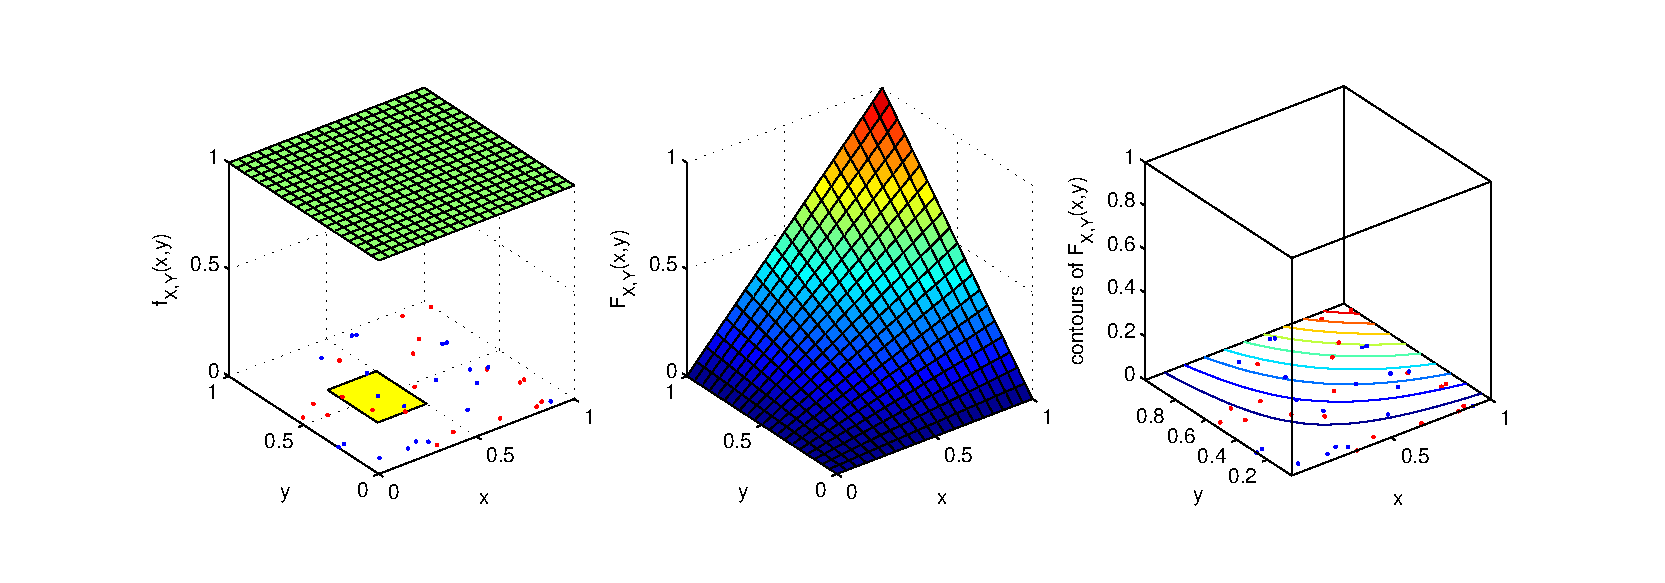
\includegraphics[width=6.5in]{figures/Unif2DPDFandCDF}}
\end{center}

Let us begin to find the needed expressions.
\be
\item
Let $(x,y) \in [0,1]^2$ then by Equation~\eqref{Eq:2ContjDFFromjPDF}:
{\small
\begin{align*}
F_{X,Y}(x,y) 
&= \int_{-\infty}^{y} \int_{-\infty}^{x} f_{X,Y}(u,v) dudv
= \int_{0}^{y} \int_{0}^{{x}} 1 dudv
= \int_{0}^{y} \left[ u \right]_{u=0}^{x}  dv
= \int_{0}^{y} x  dv
&= \left[ x v \right]_{v=0}^{y}
= {x}{y}
\end{align*}
}
\item We can obtain $\p(X \leq 1/3, Y \leq 1/2)$ by evaluating $F_{X,Y}$ at $(1/3,1/2)$:
{\small
\begin{align*}
\p(X \leq 1/3, Y \leq 1/2)
&= F_{X,Y}(1/3,1/2)
= \frac{1}{3}\frac{1}{2}
= \frac{1}{6}
\end{align*}
}
We can also find $\p(X \leq 1/3, Y \leq 1/2)$ by integrating the JPDF over the rectangular event $A=\{X < 1/3, Y < 1/2 \} \subset [0,1]^2$ according to Equation~\eqref{Eq:2ContProbEventFromjPDF}.  
This amounts here to finding the area of $A$, we compute $\p(A) = (1/3) (1/2) = 1/6$.  

\item We can find $P\left( (X,Y) \in [1/4,1/2]\times[1/3,2/3] \right)$ by integrating the JPDF over the rectangular event $B=[1/4,1/2]\times[1/3,2/3]$ according to Equation~\eqref{Eq:2ContProbEventFromjPDF}:
{\small
\begin{align*}
P\left( (X,Y) \in [1/4,1/2]\times[1/3,2/3] \right)
&=\int\int_B f_{X,Y}(x,y)dxdy
=\int_{1/3}^{2/3}\int_{1/4}^{1/2} 1 dx dy\\
&=\int_{1/3}^{2/3} \left[ x \right]_{1/4}^{1/2}  dy
=\int_{1/3}^{2/3} \left[ \frac{1}{2}-\frac{1}{4} \right]  dy
=\left(\frac{1}{2}-\frac{1}{4}\right)\left[ y \right]_{1/3}^{2/3}\\ 
&=\left(\frac{1}{2}-\frac{1}{4}\right)\left( \frac{2}{3}-\frac{1}{3} \right) 
=\frac{1}{4} \left( \frac{1}{3} \right) =\frac{1}{12}
\end{align*}
}
\ee

In general, for a bivariate uniform \rv~on the unit square the $\p([a,b]\times[c,d]) = (b-a)(d-c)$ for any event given by the rectangular region $[a,b]\times[c,d]$ inside the unit square $[0,1]\times[0,1]$.  
Thus any two events with the same rectangular area have the same probability (imagine sliding a small rectangle inside the unit square... no matter where you slide this rectangle to while remaining in the unit square, the probability of $\omega \mapsto (X(\omega),Y(\omega))=(x,y)$ falling inside this ``slidable'' rectangle is the same...).
\end{example}
 
\begin{example}\label{Eg:PlotPDF2ServerTimes}
Let the RV $X$ denote the time until a web server connects to your computer, and let the RV $Y$ denote the time until the server authorizes you as a valid user.  
Each of these RVs measures the waiting time from a common starting time (in milliseconds) and $X < Y$.  
From past response times of the web server we know that a good approximation for the JPDF of the \rv~$(X,Y)$ is
\[
f_{X,Y}(x,y) = 
\begin{cases}
\frac{6}{10^6} \exp \left( -\frac{1}{1000}x-\frac{2}{1000}y \right)
& \text{ if } x>0,y>0,x <y\\
0 & \text{ otherwise}.
\end{cases}
\]
Answer the following:
\be
\item identify the support of $(X,Y)$, i.e., the region in the plane where $f_{X,Y}$ takes positive values
\item check that $f_{X,Y}$ indeed integrates to $1$ as it should
\item Find $P(X \leq 400, Y \leq 800)$
\item It is known that humans prefer a response time of under $1/10$ seconds ($10^2$ milliseconds) from the web server before they get impatient.  What is $P(X+Y < 10^2)$? 
\ee
\begin{center}
\makebox{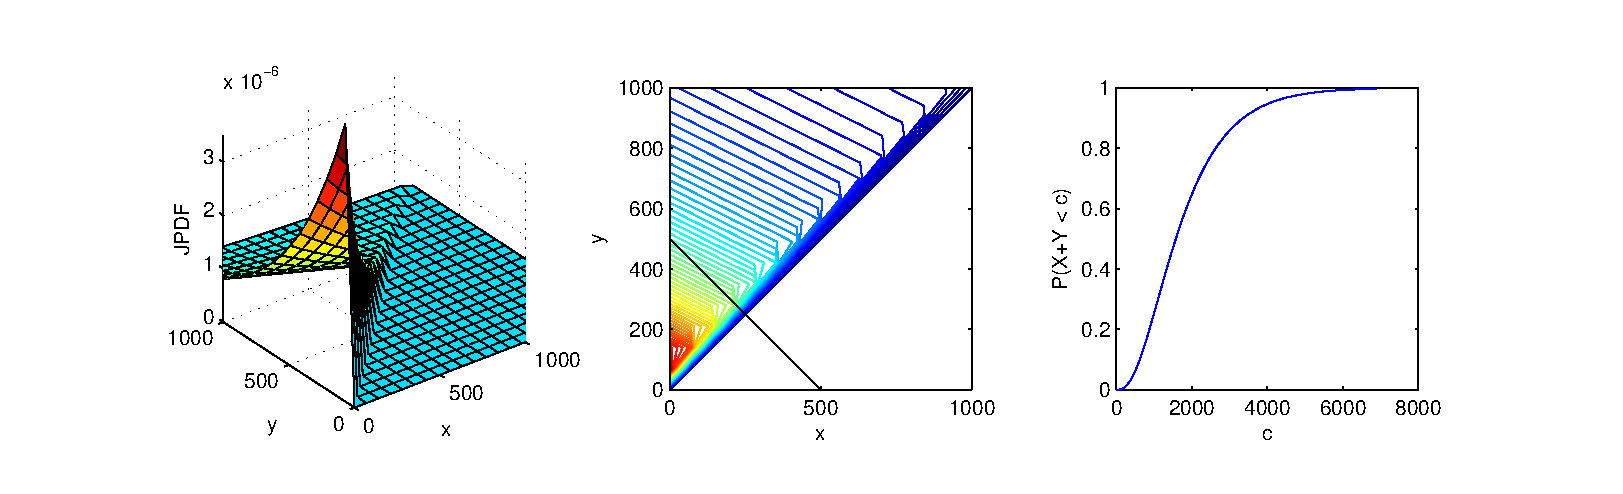
\includegraphics[width=6.0in]{figures/PlotPDF2ServerTimes}}
\end{center}
Let us answer the questions.
\be
\item
The support is the intersection of the positive quadrant with the $y>x$ half-plane.
\item
{\scriptsize
\begin{align*}
\int_{y=-\infty}^{\infty}\int_{x=-\infty}^{\infty} f_{X,Y}(x,y) dx dy 
&= \int_{x=0}^{\infty}\int_{y=x}^{\infty} f_{X,Y}(x,y) dy dx\\
&= \int_{x=0}^{\infty}\int_{y=x}^{\infty} \frac{6}{10^6} \exp \left( -\frac{1}{1000}x-\frac{2}{1000}y \right) dy dx\\
&= \frac{6}{10^6} \int_{x=0}^{\infty} \left(\int_{y=x}^{\infty} \exp \left( -\frac{2}{1000}y \right) dy \right) \exp \left(-\frac{1}{1000}x\right) dx\\
&= \frac{6}{10^6} \int_{x=0}^{\infty} \left[ -\frac{1000}{2} \exp \left( -\frac{2}{1000}y \right) \right]_{y=x}^{\infty}  \exp \left(-\frac{1}{1000}x\right) dx\\
&= \frac{6}{10^6} \int_{x=0}^{\infty} \left[0 +\frac{1000}{2}\exp \left( -\frac{2}{1000}x \right) \right]  \exp \left(-\frac{1}{1000}x\right) dx\\
&= \frac{6}{10^6} \int_{x=0}^{\infty} \frac{1000}{2}\exp \left( -\frac{2}{1000}x -\frac{1}{1000}x\right) dx\\
&= \frac{6}{10^6} \frac{1000}{2} \left[ -\frac{1000}{3} \exp \left(-\frac{3}{1000}x\right)\right]_{x=0}^{\infty} \\
&= \frac{6}{10^6} \frac{1000}{2} \left[0 +\frac{1000}{3} \right] \\
&=1
\end{align*}
}
\item
First, identify the region with positive JPDF for the event $(X \leq 400, Y \leq 800)$
{\scriptsize
\begin{align*}
&P(X \leq 400, Y \leq 800)\\
&= \int_{x=0}^{400} \int_{y=x}^{800} f_{X,Y}(x,y) dy dx \\
&= \int_{x=0}^{400} \int_{y=x}^{800} \frac{6}{10^6} \exp \left( -\frac{1}{1000}x-\frac{2}{1000}y \right) dy dx \\
&= \frac{6}{10^6}  \int_{x=0}^{400} \left[ -\frac{1000}{2} \exp \left( -\frac{2}{1000}y \right) \right]_{y=x}^{800}  \exp \left(-\frac{1}{1000}x\right) dx\\
&= \frac{6}{10^6} \frac{1000}{2} \int_{x=0}^{400} \left( - \exp \left( -\frac{1600}{1000} \right) + \exp \left( -\frac{2}{1000}x \right) \right)  \exp \left(-\frac{1}{1000}x\right) dx\\
&= \frac{6}{10^6} \frac{1000}{2} \int_{x=0}^{400} \left( \exp \left( -\frac{3}{1000}x \right) - e^{-8/5} \exp \left(-\frac{1}{1000}x\right)\right) dx\\
&= \frac{6}{10^6} \frac{1000}{2} \left( \left( -\frac{1000}{3} \exp \left( -\frac{3}{1000}x \right) \right)_{x=0}^{400} - e^{-8/5} \left(-1000 \exp \left(-\frac{1}{1000}x\right)\right)_{x=0}^{400} \right) \\
&= \frac{6}{10^6} \frac{1000}{2} 1000 \left( \frac{1}{3}\left(1- e^{-6/5} \right) - e^{-8/5} \left( 1-e^{-2/5}\right) \right) \\
&= 3 \left( \frac{1}{3}\left(1- e^{-6/5} \right) - e^{-8/5} \left( 1-e^{-2/5}\right) \right) \\
&\approxeq 0.499 \enspace .
\end{align*}
}
\item
First, identify the region with positive JPDF for the event $(X+Y \leq c)$, say $c=500$ (but generally $c$ can be any positive number).
This is the triangular region at the intersection of the four half-planes: $x>0$, $x < c$, $y>x$ and $y<c-x$. ({\em Draw picture here})
%\vspace{2cm}\\
Let's integrate the JPDF over our triangular event as follows:
{\scriptsize
\begin{align*}
P(X+Y \leq c) 
&= \int_{x=0}^{c/2}\int_{y=x}^{c-x} f_{X,Y}(x,y) dy dx \\
&= \int_{x=0}^{c/2}\int_{y=x}^{c-x} \frac{6}{10^6} \exp \left( -\frac{1}{1000}x-\frac{2}{1000}y \right) dy dx \\
&= \frac{6}{10^6} \int_{x=0}^{c/2}\int_{y=x}^{c-x}  \exp \left( -\frac{1}{1000}x-\frac{2}{1000}y \right) dy dx \\
&= \frac{6}{10^6} \frac{1000}{2} \int_{x=0}^{c/2} \left[ - \exp \left( -\frac{2}{1000}y \right) \right]_{y=x}^{c-x}  \exp \left(-\frac{1}{1000}x\right) dx\\
&= \frac{3}{10^3} \int_{x=0}^{c/2} \left[ - \exp \left( -\frac{2c-2x}{1000} \right) + \exp \left( -\frac{2x}{1000} \right) \right]  \exp \left(-\frac{x}{1000}\right) dx\\
&= \frac{3}{10^3} \int_{x=0}^{c/2} \left(  \exp \left( -\frac{3x}{1000} \right) - \exp \left( \frac{x-2c}{1000} \right) \right)  dx\\
&= 3 \left( \left[-\frac{1}{3} \exp \left( -\frac{3x}{1000} \right) \right]_{x=0}^{c/2} - \left[ e^{-2c/1000} \exp \left( \frac{x}{1000} \right)\right]_{x=0}^{c/2} \right)  \\
&= 3  \left(\frac{1}{3} (1-e^{-3c/2000}) - e^{-2c/1000} (e^{c/2000}-1) \right)\\
&= 1 - e^{-3c/2000} + 3 e^{-2c/1000} - 3 e^{-3c/2000}\\
&= 1 - 4 e^{-3c/2000} + 3 e^{-c/500}
\end{align*}
}
%\vspace{1cm}\\
\item $P(X+Y<100) = 1 - 4 e^{-300/2000} + 3 e^{-100/500} \approxeq 0.134$.  This means only about one in one hundred requests to this server will be processed within 100 milliseconds.
\ee
We can obtain $P(X+Y<c)$ for several values of $c$ using \Matlab and note that about 96\% of requests are processed in less than 3000 milliseconds or 3 seconds.
\begin{VrbM}
>> c = [100 1000 2000 3000 4000]
c =  100        1000        2000        3000        4000

>> p = 1 - 4 * exp(-3*c/2000) + 3 * exp(-c/500)

p =  0.0134     0.5135      0.8558      0.9630      0.9911
\end{VrbM}
\end{example}

\begin{definition}[Marginal PDF or PMF]
If the \rv~$(X,Y)$ has $f_{X,Y}(x,y)$ as its joint PDF or joint PMF, then the 
{\bf marginal PDF or PMF} of a random vector $(X,Y)$ is defined by :
\[
f_{X}(x) =
\begin{cases}
\int_{-\infty}^{\infty} f_{X,Y}(x,y) dy & \text{if $(X,Y)$ is a continuous \rv}  \\
\sum_{y} f_{X,Y}(x,y) & \text{if $(X,Y)$ is a discrete \rv} \\
\end{cases}
\]
and the  {\bf marginal PDF or PMF} of $Y$ is defined by:
\[
f_{Y}(y) = 
\begin{cases}
\int_{-\infty}^{\infty} f_{X,Y}(x,y) dx & \text{if $(X,Y)$ is a continuous \rv}  \\
\sum_{x} f_{X,Y}(x,y) & \text{if $(X,Y)$ is a discrete \rv} \\
\end{cases}
\]
\end{definition}

\begin{example}
Obtain the marginal PMFs $f_Y(y)$ and $f_X(x)$ from the joint PMF $f_{X,Y}(x,y)$ of the discrete \rv~in \hyperref[Eg:Discrete2DPMF]{Example~\ref*{Eg:Discrete2DPMF}}.
Just sum $f_{X,Y}(x,y)$ over $x$'s and $y$'s (reported in a tabular form):
\begin{center}
\begin{tabular}{|c|c c|}
\hline
& $Y=0$ & $Y=1$ \\ \hline
$X=0$& $0.1$ & $0.3$  \\
$X=1$& $0.2$ & $0.4$  \\ \hline
\end{tabular}
\end{center}
From the above Table we can find:
\begin{align*}
f_X(x) = P(X=x) 
&= \sum_{y} f_{X,Y}(x,y) \\
&= 
f_{X,Y}(x,0) + f_{X,Y}(x,1) = 
\begin{cases}
f_{X,Y}(0,0) + f_{X,Y}(0,1) = 0.1+0.3=0.4 & \text{ if } x=0\\
f_{X,Y}(1,0) + f_{X,Y}(1,1) = 0.2+0.4=0.6 & \text{ if } x=1\\
\end{cases}
\end{align*}
Similarly,
\begin{align*}
f_Y(y) = P(Y=y) 
&= \sum_{x} f_{X,Y}(x,y) \\
&= 
f_{X,Y}(0,y) + f_{X,Y}(1,y) 
= 
\begin{cases}
f_{X,Y}(0,0) + f_{X,Y}(1,0) = 0.1+0.2=0.3 & \text{ if } y=0\\
f_{X,Y}(0,1) + f_{X,Y}(1,1) = 0.3+0.4=0.7 & \text{ if } y=1\\
\end{cases}
\end{align*}
Just report the marginal probabilities as row and column sums of the JPDF table.

Thus marginal PMF gives us the probability of a specific RV, within a \rv, taking a value irrespective of the value taken by the other RV in this \rv. 
\end{example}

\begin{example}
Obtain the marginal PDFs $f_Y(y)$ and $f_X(x)$ from the joint PDF $f_{X,Y}(x,y)$ of the continuous \rv~in \hyperref[Eg:Unif2DPDFandCDF]{Example~\ref*{Eg:Unif2DPDFandCDF}} (the bivariate uniform \rv~on $[0,1]^2$).

\begin{center}
\makebox{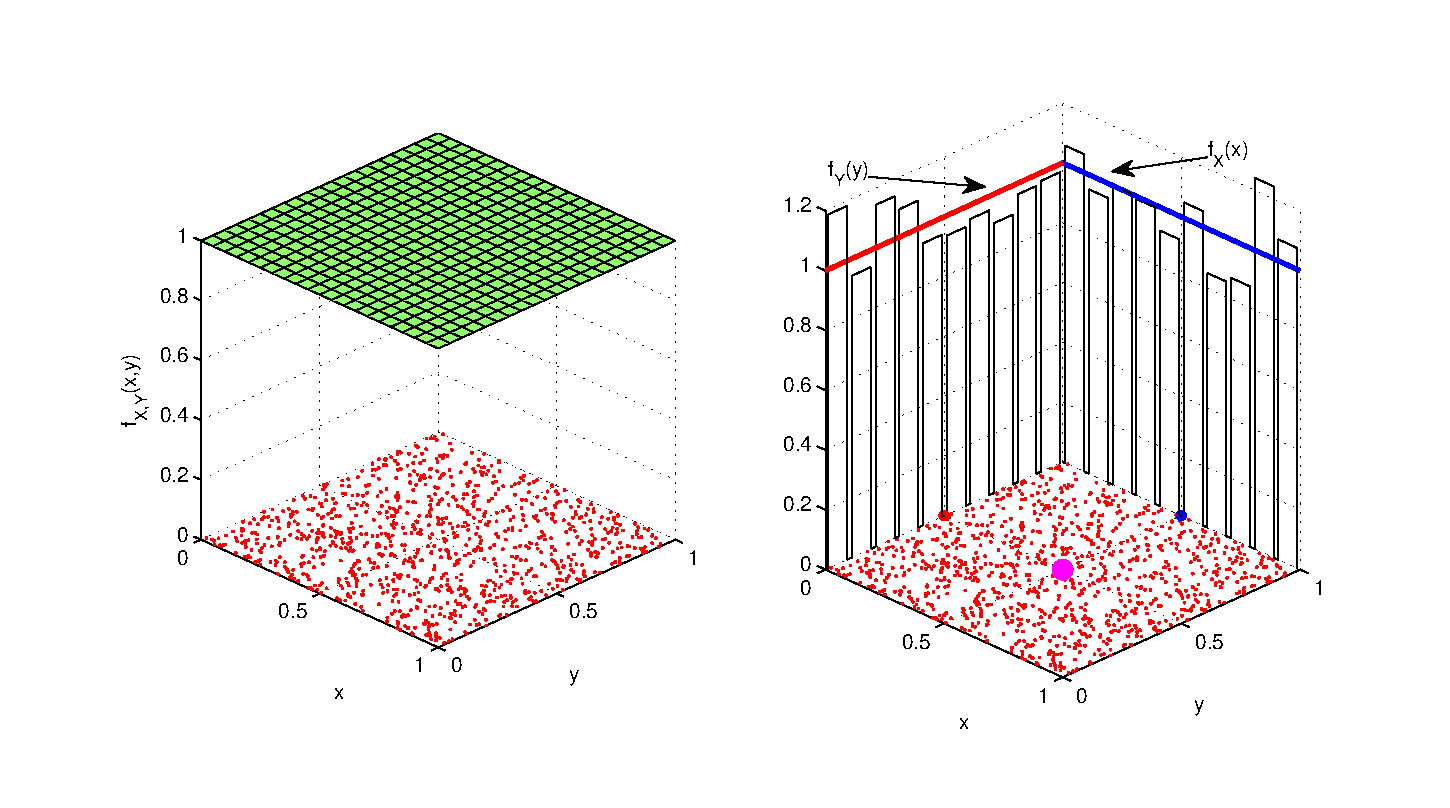
\includegraphics[width=6.0in]{figures/PlotPDFSamplesMarginalsUnif2D}}
\end{center}

Let us suppose $(x,y) \in [0,1]^2$ and note that $f_{X,Y}=0$ if $(x,y) \notin [0,1]^2$.  
We can obtain marginal PMFs $f_X(x)$ and $f_Y(y)$ by integrating the JPDF $f_{X,Y}=1$ along $y$ and $x$, respectively.
\[
f_X(x) = \int_{-\infty}^{\infty} f_{X,Y}(x,y) dy = \int_{0}^{1} f_{X,Y}(x,y) dy 
= \int_{0}^{1} 1 dy = \left[ y \right]_0^1 = 1-0 = 1
\]
Similarly,
\[
f_Y(y) = \int_{-\infty}^{\infty} f_{X,Y}(x,y) dx = \int_{0}^{1} f_{X,Y}(x,y) dx 
= \int_{0}^{1} 1 dx = \left[ x \right]_0^1 = 1-0 = 1
\]
We are seeing a histogram of the {\bf marginal samples} and their marginal PDFs in the Figure.
\end{example}

Thus marginal PDF gives us the probability density of a specific RV in a \rv, irrespective of the value taken by the other RV in this \rv. 

\begin{example}
Obtain the marginal PDF $f_Y(y)$ from the joint PDF $f_{X,Y}(x,y)$ of the continuous \rv~in \hyperref[Eg:PlotPDF2ServerTimes]{Example~\ref*{Eg:PlotPDF2ServerTimes}} that gave the response times of a web server.
\[
f_{X,Y}(x,y) = 
\begin{cases}
\frac{6}{10^6} \exp \left( -\frac{1}{1000}x-\frac{2}{1000}y \right)
& \text{ if } x>0,y>0,x <y\\
0 & \text{ otherwise}.
\end{cases}
\]
Use $f_Y(y)$ to compute the probability that $Y$ exceeds 2000 milliseconds.

%\vspace{5in}
First we need to obtain an expression for $f_Y(y)$. For $y > 0$,
{\scriptsize
\begin{align*}
f_Y(y) 
&= \int_{x=-\infty}^{\infty} f_{X,Y}(x,y) dx\\
&= \int_{x=-\infty}^{\infty} 6 \times 10^{-6} e^{-0.001 x - 0.002y} dx\\
&= 6 \times 10^{-6} \int_{x=0}^{y} e^{-0.001 x - 0.002y} dx\\ 
&= 6 \times 10^{-6} e^{-0.002y} \int_{x=0}^{y}  e^{-0.001 x} dx\\ 
&= 6 \times 10^{-6} e^{-0.002y} \left[ \frac{e^{-0.001 x}}{-0.001}\right]_{x=0}^{x=y}\\ 
&= 6 \times 10^{-6} e^{-0.002y} \left( \frac{e^{-0.001 y}}{-0.001} - \frac{e^{-0.001 \times 0}}{-0.001} \right)\\ 
&= 6 \times 10^{-6} e^{-0.002y} \left( \frac{1- e^{-0.001 y}}{0.001} \right)\\ 
&= 6 \times 10^{-3} e^{-0.002y} \left({1- e^{-0.001 y}} \right)\\ 
\end{align*}
}
We have the marginal PDF of $Y$ and from this we can obtain 
{\scriptsize
\begin{align*}
P(Y>2000)
&= \int_{2000}^{\infty} f_Y(y) dy \\
&= \int_{2000}^{\infty} 6 \times 10^{-3} e^{-0.002y} \left({1- e^{-0.001 y}} \right) dy\\
&= 6 \times 10^{-3} \int_{2000}^{\infty}  e^{-0.002y} dy - \int_{2000}^{\infty} e^{-0.003 y} dy\\
&= 6 \times 10^{-3} \left( \left[ \frac{e^{-0.002y}}{-0.002} \right]_{2000}^{\infty} 
- \left( \left[ \frac{e^{-0.003y}}{-0.003} \right]_{2000}^{\infty} \right) \right)\\
&= 6 \times 10^{-3} \left( \frac{e^{-4}}{0.002} - \frac{e^{-6}}{0.003} \right)\\
&= 0.05
\end{align*}
}

{\scriptsize
Alternatively, you can obtain $P(Y>2000)$ by directly integrating the joint PDF $f_{X,Y}(x,y)$ over the appropriate region (but you may now have to integrate two pieces: rectangular infinite strip ${(x,y): 0<x<2000, y>2000}$ and a triangular infinite piece $\{(x,y): y>x, y>2000, x> 2000\}$)... more involved but we get the same answer.
\begin{multline*}
P(Y>2000) = \int_{x=0}^{2000} \left( \int_{y=2000}^{\infty} 6 \times 10^{-6} e^{-0.001 x - 0.002y} dy \right) dx + \\
\int_{x=2000}^{\infty} \left( \int_{y=x}^{\infty} 6 \times 10^{-6} e^{-0.001 x - 0.002y} dy \right) dx 
\\
\vdots \text{(try as a tutorial problem)} \\
P(Y>2000) = 0.0475 + 0.0025 = 0.05
\end{multline*}
}
\end{example}

We have seen the notion of independnece of two events in \hyperref[D:IndOf2Events]{Definition~\ref*{D:IndOf2Events}} or of a sequence of events in \hyperref[D:IndOfSeqOfEvents]{Definition~\ref*{D:IndOfSeqOfEvents}}. 
Recall that independence amounts to having the probability of the joint occurrence of the events to be given by the product of the probabilities of each of the events.

We can use the definition of independence of two events to define the independence of two random variables using their distribution functions.

\begin{definition}[Independence of Two RVs]\label{D:Ind2RVs}
Consider an $\Rz^2$-valued RV $X:=(X_1,X_2)$. Then the $\Rz$-valued RVs $X_1$ and $X_2$ are said to be independent or independently distributed if and only if
\[
\p(X_{1} \leq x_{1}, X_{2} \leq x_{2} ) = \p(X_{1} \leq x_{1}) \p(X_{2} \leq x_{2})
\]
or equivalently,
\[
F_{X_{1},X_{2}}(x_{1},x_{2}) = F_{X_{1}}(x_{1}) F_{X_{2}}(x_{2}) \enspace ,
\]
for any pair of real numbers $(x_{1},x_{2}) \in \Rz^2$.

By the above definition, for {\bf discrete} RVs $X_1,X_2$ that are independent, the following equality is satisfied between the joint and marginal PMFs:
\[
f_{X_1,X_2}(x_1,x_2) = \p(X_{1}= x_{1}, X_{2} = x_{2}) = \p(X_{1} = x_{1}) \p(X_{2} = x_{2}) = f_{X_1}(x_1) f_{X_2}(x_2) \text{ for any} (x_{1},x_{2}) \in \Rz^2 \enspace ,
\]
and for {\bf continuous} RVs $X_1,X_2$ that are independent, the following equality is satisfied between the joint and marginal PDFs:
\[
f_{X_1,X_2}(x_1,x_2) = f_{X_1}(x_1) f_{X_2}(x_2)  \text{ for any} (x_{1},x_{2}) \in \Rz^2 \enspace .
\] 
\end{definition}

In summary, two RVs $X$ and $Y$ are said to be {\bf independent} if and only if for every $(x,y)$
\[
\boxed{
F_{X,Y}(x,y) = F_X(x) \times F_Y(y) \qquad \text{ or } f_{X,Y}(x,y) = f_X(x) \times f_Y(y)
}
\]

Let us confirm that our familiar experiment of tossing a fair coin twice independently when encoded by a pair of independent $\bernoulli(1/2)$ RVs satisfies the above definition.
\begin{example}[Pair of independent $\bernoulli(1/2)$ RVs]
Let $X_1$ and $X_2$ be a pair of independent $\bernoulli(1/2)$ RVs each taking values in the set $\{0,1\}$ with the following tabulated probabilities. Verify that the JPMF $f_{X_1,X_2}(x_1,x_2)=1/4$ for each $(x_1,x_2) \in \{0,1\}^2$ is indeed given by the marginal PMF $f_{X_i}(x_i)=1/2$ for each $i \in \{1,2\}$ and each $x_i \in \{0,1\}$.

\begin{center}
\begin{tabular}{|c|c c|c|}
\hline
& $X_2=0$ & $X_2=1$ & \\ \hline
$X_1=0$& $1/4$ & $1/4$ & $1/2$ \\
$X_1=1$& $1/4$ & $1/4$ & $1/2$ \\ \hline
& $1/2$ & $1/2$ & $1$\\ \hline
\end{tabular}
\end{center}
From the above Table we can read for instance that the {\em joint probability} that $\Rz^2$-valued RV $(X_1,X_2)$ takes the value or realization $(0,0)$ is $1/4$ from the first entry of the inner-most tabulated rectangle, 
i.e., $\p((X_1,X_2)=(0,0))=1/4$, 
and that the {\em marginal probability} that the RV $X_1$ takes the value or relaization $0$ is $1/2$, 
i.e., $\p(X_1=0)=1/2$. 
Clearly, $1/4=1/2 \times 1/2$, and so our familiar experiment when seen as an $\Rz^2$-valued RV is indeed composed of two independent$\Rz$-valued $\bernoulli(1/2)$ RVs. 
\end{example}

\begin{example}
Recall the $\Rz^2$-valued continuous RV $(X,Y)$ of \hyperref[Eg:Unif2DPDFandCDF]{Example~\ref*{Eg:Unif2DPDFandCDF}} 
that is uniformly distributed on the unit square $[0,1]^2$. 
First show that $X$ and $Y$ independent. 
Then show that both $X$ and $Y$ are identically distributed according to the $\uniform(0,1)$ RV. 

This can be shown by checking that the joint PDF is indeed equal to the product of the marginal PDFs of $\uniform(0,1)$ RVs as follows:
\[
\begin{cases}
1= f_{X,Y}(x,y) =  f_X(x) \times f_Y(y) = 1 \times 1 = 1 & \text{ if } (x,y) \in [0,1]^2\\
0= f_{X,Y}(x,y) =  f_X(x) \times f_Y(y) = 0 \times 0 = 0 & \text{ if } (x,y) \notin [0,1]^2
\end{cases}
\]
\end{example}

Are $X$ and $Y$ independent in the server times \rv~from \hyperref[Eg:PlotPDF2ServerTimes]{Example~\ref*{Eg:PlotPDF2ServerTimes}}?

We can compute $f_X(x)$ and use the already computed $f_Y(y)$ to mechanically check if the JPDF is the product of the marginal PDFs.  But intuitively, we know that these RVs (connection time and authentication time) are dependent -- one is strictly greater than the other.  
Also the JPDF has zero density when $x>y$, but the product of the marginal densities won't.

Now, let us take advantage of independent random variables and solve some problems.

\begin{example}[distance between random faults in a manufactured line]
Suppose two points are tossed independently and uniformly at random onto a line segment of unit length.  
What is the probability that the distance between the two points does not exceed a given length $l$? 

\vspace{5cm}
done in lectures...

\end{example}

Let us introduce parameters for the lower and upper bounds of the interval upon which a continuous RV is uniformly distributed using the following probability model.
 
\begin{model}[$\uniform(\theta_1,\theta_2)$]\label{M:Uniformab}
Given two real parameters $\theta_1,\theta_2 \in \Rz$, such that $\theta_1 < \theta_2$, the PDF of the $Uniform(\theta_1,\theta_2)$ RV $X$ is:
\begin{equation}\label{E:Uniformabpdf}
f(x;\theta_1,\theta_2) =
\begin{cases}
\frac{1}{\theta_2 - \theta_1} & \text{if $\theta_1 \leq x \leq \theta_2$,}\\
0 & \text{otherwise}
\end{cases}
\end{equation}
and its DF given by $F(x;\theta_1,\theta_2) = \int_{- \infty}^x f(y; \theta_1,\theta_2) \, dy$ is:
\begin{equation}\label{E:Uniformabcdf}
F(x; \theta_1,\theta_2) =
\begin{cases}
0 & \text{if $x < \theta_1$} \\
\frac{x-\theta_1}{\theta_2-\theta_1} & if~\theta_1 \leq x \leq \theta_2,\\
1 & \text{if $x > \theta_2$}
\end{cases}
\end{equation}
Recall that we emphasise the dependence of the probabilities on the two parameters $\theta_1$ and $\theta_2$ by specifying them following the semicolon in the argument for $f$ and $F$.
\end{model}
\begin{figure}[htpb]
\caption{A plot of the PDF, DF or CDF and inverse DF of the $\uniform(-1,1)$ RV $X$.\label{F:unifpm1}}
\centering   \makebox{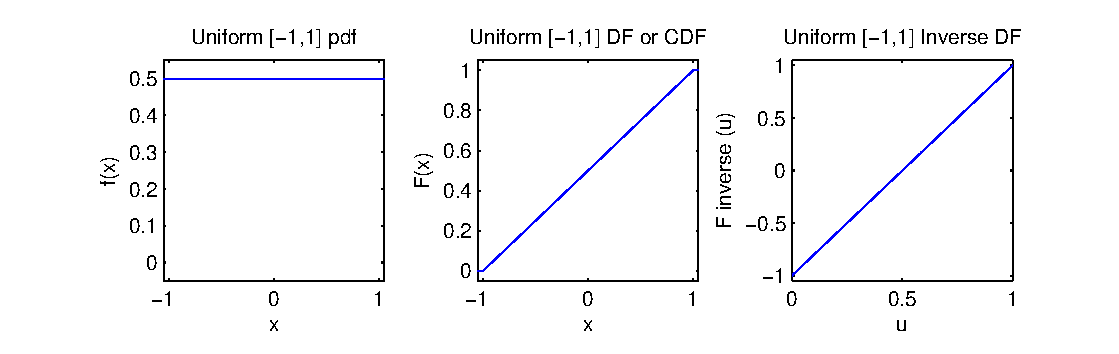
\includegraphics[width=6.5in]{figures/Unifpm1pdfcdf}}
\end{figure}
\begin{example}[Buffon's Needle Experiment to Physically Estimate $\pi$]
~

done in lectures...
\vspace{5cm}

\end{example}

\subsection{Conditional Random Variables}

Often we will have a condition where one of the two random variables that make up a random vector $(X_1,X_2)$ already occurs and takes a value. 
And we might want to compute the probability of the occurrence of the other random variable given this conditional information.
For this all we need to do is extend the idea of conditional probabiliies to $\Rz^2$-valued random variables as defined below.

\begin{definition}[Conditional PDF or PMF]
Let $(X_1,X_2)$ be a discrete bivariate \rv.  The conditional PMF of $X_1|X_2=x_2$, where $f_{X_2}(x_2) := \p(X_2=x_2) > 0$ is:
\[
f_{X_1|X_2}(x_1 | x_2) := \p(X_1=x_1 | X_2=x_2) = \frac{\p(X_1=x_1,X_2=x_2)}{\p(X_2=x_2)} = \frac{f_{X_1,X_2}(x_1,x_2)}{f_{X_2}(x_2)} \ .
\]
Similarly, if $f_{X_1}(x_1) := \p(X_1=x_1) >0$, then the conditional PMF of $X_2|X_1=x_1$ is:
\[
f_{X_2|X_1}(x_2|x_1) := \p(X_2=x_2 | X_1=x_1) = \frac{\p(X_1=x_1,X_2=x_2)}{\p(X_1=x_1)} = \frac{f_{X_1,X_2}(x_1,x_2)}{f_{X_1}(x_1)} \ .
\]
If $(X_1,X_2)$ are continuous RVs such that the marginal PDF $f_{X_2}(x_2)>0$, then the conditional PDF of $X_1|X_2=x_2$ is:
\[
f_{X_1|X_2}(x_1|x_2) = \frac{f_{X_1,X_2}(x_1,x_2)}{f_{X_2}(x_2)}, \qquad \p(X_1 \in A| X_2=x_2) = \int_A f_{X_1|X_2}(x_1|x_2) dx_1 \ .
\]
Similarly, if $f_{X_1}(x_1)>0$, then the conditional PDF of $X_2|X_1=x_1$ is:
\[
f_{X_2|X_1}(x_2|x_1) = \frac{f_{X_1,X_2}(x_1,x_2)}{f_{X_1}(x_1)}, \qquad \p(X_2 \in A| X_1=x_1) = \int_A f_{X_2|X_1}(x_2|x_1) dx_2 \ .
\]
\end{definition}

Let us consider a few discrete RVs for the simple coin tossing experiment $\E{E}_{\theta}^{3}$ that build on the $\bernoulli(\theta)$ RV $X_i$ for the $i$-th toss in an {\bf independent and identically distibuted (IID.)} manner.
\begin{table}[htpb]
\caption{The $8$ $\omega$'s in the sample space $\Omega$ of the experiment $\E{E}_{\theta}^{3}$ are given in the first row above.  The RV $Y$ is the number of `Heads' in the $3$ tosses and the RV $Z$ is the number of `Tails' in the $3$ tosses.  Finally, the RVs $Y'$ and $Z'$ are the indicator functions of the event that `all three tosses were Heads' and the event that `all three tosses were Tails', respectively.\label{T:T3XRVs}}
 \begin{tabular}{r c c c c c c c c l}
 \hline
$\omega$:    & {\tt HHH} & {\tt HHT} & {\tt HTH} & {\tt HTT} & {\tt THH} & {\tt THT} & {\tt TTH} & {\tt TTT} & RV Definitions / Model \\ \hline
 \\
$\p(\omega)$: & $\frac{1}{8}$ & $\frac{1}{8}$ & $\frac{1}{8}$ & $\frac{1}{8}$ &  $\frac{1}{8}$ & $\frac{1}{8}$ & $\frac{1}{8}$ & $\frac{1}{8}$  & $X_i \overset{\IID}{\sim} \bernoulli(\frac{1}{2})$ \\
 \\
$Y(\omega)$: & 3         & 2         & 2         & 1         & 2         & 1         & 1         & 0        & $Y := X_1+X_2+X_3$ \\
 \\
$Z(\omega)$: & 0         & 1         & 1         & 2         & 1         & 2         & 2         & 3        & $Z := (1-X_1)+(1-X_2)+(1-X_3)$ \\
 \\
$Y'(\omega)$: & 1         & 0         & 0         & 0         & 0         & 0         & 0         & 0       & $Y' :=  X_1 X_2 X_3$ \\
\\
$Z'(\omega)$: & 0         & 0         & 0         & 0         & 0         & 0         & 0         & 1       & $Y' :=  (1-X_1)(1-X_2)(1-X_3)$ \\ \hline
 \end{tabular}
 \end{table}
 \begin{classwork}[Two random variables of `toss a coin thrice' experiment]
Describe the probability of the RV $Y$ and $Y'$ of \hyperref[T:T3XRVs]{Table \ref*{T:T3XRVs}} in terms of its PMF.  Repeat the process for the RV $Z$ in your spare time.
 \begin{eqnarray}
 \p(Y=y) =%:= \p(\{\omega: Y(\omega)=y\}) = 
 \begin{cases}
 \qquad & \qquad \notag \\
 \qquad & \qquad \notag \\
 \qquad & \qquad \notag \\
 \qquad & \qquad \notag
 \end{cases} 
 & \qquad \qquad \qquad \qquad \qquad
\p(Y'=y') =%:= \p(\{\omega: Y'(\omega)=y'\}) = 
 \begin{cases}
 \qquad & \qquad \notag \\
 \qquad & \qquad \notag 
 \end{cases}
 \end{eqnarray}
 \end{classwork}
 
 \begin{classwork}[The number of `Heads' given there is at least one `Tails']
 Consider the following two questions.
 \begin{enumerate}
\item What is conditional probability $\p(Y|Y'=0)$ ?
%{\color{Gray}{
 \[
 \begin{array}{c c c c}
 \hline \\
 \p(Y=y | Y'=0) & =\frac{\p(Y=y,Y'=0)}{\p(Y'=0)} & =\frac{\p(\{\omega: Y(\omega)=y \  \cap \ Y'(\omega)=0\})}{\p(\{\omega: Y'(\omega)=0\})} & = ? \\ \hline \\
 \\
 \p(Y=0 | Y'=0) & \frac{\p(Y=0,Y'=0)}{\p(Y'=0)} & \frac{\frac{1}{8}}{\frac{1}{8}+\frac{1}{8}+\frac{1}{8}+\frac{1}{8}+\frac{1}{8}+\frac{1}{8}+\frac{1}{8}} & \frac{1}{7} \\
\\
\p(Y=1 | Y'=0) & \frac{\p(Y=1,Y'=0)}{\p(Y'=0)} & \frac{\frac{1}{8}+\frac{1}{8}+\frac{1}{8}}{\frac{1}{8}+\frac{1}{8}+\frac{1}{8}+\frac{1}{8}+\frac{1}{8}+\frac{1}{8}+\frac{1}{8}} & \frac{3}{7} \\
\\
\p(Y=2 | Y'=0) & \frac{\p(Y=2,Y'=0)}{\p(Y'=0)} & \frac{\frac{1}{8}+\frac{1}{8}+\frac{1}{8}}{\frac{1}{8}+\frac{1}{8}+\frac{1}{8}+\frac{1}{8}+\frac{1}{8}+\frac{1}{8}+\frac{1}{8}} & \frac{3}{7} \\
\\
\p(Y=3 | Y'=0) & \frac{\p(Y=3,Y'=0)}{\p(Y'=0)} & \frac{\p(\emptyset)}{\frac{1}{8}+\frac{1}{8}+\frac{1}{8}+\frac{1}{8}+\frac{1}{8}+\frac{1}{8}+\frac{1}{8}} & 0 \\
\\ \hline
\p(Y \in \{0,1,2,3\} | Y'=0) & \frac{\sum_{y=0}^3{\p(Y=y,Y'=0)}}{\p(Y'=0)} & \frac {\frac{1}{8}+\frac{1}{8}+\frac{1}{8}+\frac{1}{8}+\frac{1}{8}+\frac{1}{8}+\frac{1}{8}}{\frac{1}{8}+\frac{1}{8}+\frac{1}{8}+\frac{1}{8}+\frac{1}{8}+\frac{1}{8}+\frac{1}{8}} & 1 \\ \hline
 \end{array}
 \]
% }}
\item What is $\p(Y|Y'=1)$ ?
%{\color{Gray}{
 \[
\p(Y=y | Y'=1) = 
\begin{cases}
1 & \text{if $y=3$} \\
0 & \text{otherwise}
 \end{cases}
 \]
 %}}
 \end{enumerate}
 \end{classwork}

\subsection{$\Rz^m$-valued Random Variables}

%Extension to multivariate random vectors that are made of more than two RVs is straightforward.  
Consider the \rv~ $X$ whose components are the RVs $X_1,X_2,\ldots,X_m$, i.e., $X := (X_1,X_2,\ldots,X_m)$, where $m \geq 2$.  
A particular realization of this RV is a point $(x_1,x_2,\ldots,x_m)$ in $\Rz^m$.  
Now, let us extend the notions of JCDF, JPMF and JPDF to $\Rz^m$.  

\begin{definition}[multivariate JDF]\label{Df:JmDF}
The {\bf joint distribution function (JDF)} or {\bf joint cumulative distribution function (JCDF)}, $F_{X_1,X_2,\ldots,X_m}(x_1,x_2,\ldots,x_m):\mathbb{R}^m\to [0,1]$, of the multivariate random vector $(X_1,X_2,\ldots,X_m)$ is
\begin{eqnarray}\label{E:jmDF}
F_{X_1,X_2,\ldots,X_m}(x_1,x_2,\ldots,x_m)\; 
&=& P(X\leq x_1 \cap X_2 \leq x_2 \cap \cdots \cap X_m \leq x_m)\notag\\ 
&=& P(X_1\leq x_1 , X_2 \leq x_2, \ldots, X_m \leq x_m)\\
&=& P\left( \{ \omega: X_1(\omega) \leq x_1, X_2(\omega) \leq x_2, \ldots, X_m(\omega) \leq x_m \} \right), \notag
\end{eqnarray}
for any $(x_1,x_2,\ldots,x_m) \in \mathbb{R}^m$, 
where the right-hand side represents the probability that the random vector $(X_1,X_2,\ldots,X_m)$ takes on a value in 
$\{(x'_1,x'_2,\ldots,x'_m): x'_1 \leq x_1, x'_2 \leq x_2, \ldots, x'_m \leq x_m\}$, the set of points in $\Rz^m$ that are less than the point $(x_1,x_2,\ldots,x_m)$ in each coordinate $1,2,\ldots,m$.
\end{definition}

The JDF $F_{X_1,X_2,\ldots,X_m}(x_1,x_2,\ldots,x_m):\Rz^m\to\Rz$ satisfies the following conditions to remain a probability: 
\begin{enumerate}
\item $0 \leq F_{X_1,X_2,\ldots,X_m}(x_1,x_2,\ldots,x_m) \leq 1$
\item $F_{X_1,X_2,\ldots,X_m}(x_1,x_2,\ldots,x_m)$ is an increasing function of $x_1$, $x_2$, $\ldots$ and $x_m$
\item $F_{X_1,X_2,\ldots,X_m}(x_1,x_2,\ldots,x_m) \to 1$ as $x_1\to \infty$, $x_2\to \infty$, $\ldots$ and $x_m\to \infty$
\item $F_{X_1,X_2,\ldots,X_m}(x_1,x_2,\ldots,x_m) \to 0$ as $x_1\to -\infty$, $x_2\to -\infty$, $\ldots$ and $x_m\to -\infty$
\end{enumerate}

\begin{definition}[Multivariate JPMF]
If $(X_1,X_2,\ldots,X_m)$ is a {\bf discrete random vector} that takes values in a discrete support set $\mathcal{S}_{X_1,X_2,\ldots,X_m}$, then its \textbf{joint probability mass function} (or JPMF) is:
\begin{equation}\label{Eq:jmDPMF}
f_{X_1,X_2,\ldots,X_m}(x_1,x_2,\ldots,x_m) = P(X_1=x_1,X_2=x_2,\ldots,X_m=x_m) \enspace . 
\end{equation}
\end{definition}
Since $P(\Omega)=1$, $\sum_{{\substack{(x_1,x_2,\ldots,x_m) \in \mathcal{S}_{X_1,X_2,\ldots,X_m}}}}f_{X_1,X_2,\ldots,X_m}(x_1,x_2,\ldots,x_m)=1$.

From JPMF $f_{X_1,X_2,\ldots,X_m}$ we can get the JCDF $F_{X_1,X_2,\ldots,X_m}(x_1,x_2,\ldots,x_m)$ and the probability of any event $B$ by simply taking sums as in Equation~\eqref{Eq:2DiscretejDFFromjPMF} but now over all $m$ coordinates.
%\begin{equation}\label{Eq:2DiscretejDFFromjPMF}
%\boxed{F_{X_1,X_2,\ldots,X_m}(x,y)\;=\;\sum_{x_i\leq x, y_j \leq y}f_{X_1,X_2,\ldots,X_m}(x_i,y_j) }\enspace ,
%\qquad \boxed{P(B)\;=\;\sum_{\substack{(x_i, y_j) \in B \cap \mathcal{S}_{X_1,X_2,\ldots,X_m}}}f_{X_1,X_2,\ldots,X_m}(x_i,y_j) }\enspace ,
%\end{equation}

\begin{definition}[Multivariate JPDF]
$(X_1,X_2,\ldots,X_m)$ is a {\bf continuous random vector} if its JDF $F_{X_1,X_2,\ldots,X_m}(x_1,x_2,\ldots,x_m)$ is differentiable and the {\bf joint probability density function (JPDF)} is given by:
\[
f_{X_1,X_2,\ldots,X_m}(x_1,x_2,\ldots,x_m) = \frac{\partial^m}{\partial x_1 \partial x_2 \cdots \partial x_m} F_{X_1,X_2,\ldots,X_m}(x_1,x_2,\ldots,x_m) \enspace ,
\]
\end{definition}

From JPDF $f_{X_1,X_2,\ldots,X_m}$ we can compute the JDF $F_{X_1,X_2,\ldots,X_m}$ at any point $(x_1,x_2,\ldots,x_m) \in \Rz^m$ and more generally we can compute the probability of any event $B$, that can be cast as a region in $\Rz^m$, by ``simply'' taking $m$-dimensional integrals (you have done such iterated integrals when $m=3$):
\begin{equation}\label{Eq:mContjDFFromjPDF}
\boxed{F_{X_1,X_2,\ldots,X_m}(x_1,x_2,\ldots,x_m) = \int_{-\infty}^{x_m} \cdots \int_{-\infty}^{x_2} \int_{-\infty}^{x_1} f_{X_1,X_2,\ldots,X_m}(x_1,x_2,\ldots,x_m) dx_1 dx_2\ldots d x_m}\enspace ,
\end{equation}
and
\begin{equation}\label{Eq:mContProbEventFromjPDF}
\boxed{P(B)\;=\; \int\cdots\int\int_{B} f_{X_1,X_2,\ldots,X_m}(x_1,x_2,\ldots,x_m) dx_1 dx_2\ldots d x_m}\enspace .
\end{equation}
The JPDF satisfies the following two properties:
\be
\item integrates to $1$, i.e., $\int_{-\infty}^{\infty} \cdots \int_{-\infty}^{\infty}\int_{-\infty}^{\infty} f_{X_1,X_2,\ldots,X_m}(x_1,x_2,\ldots,x_m) dx_1 dx_2\ldots d x_m=1$
\item is a non-negative function, i.e., $f_{X_1,X_2,\ldots,X_m}(x_1,x_2,\ldots,x_m) \geq 0$.
\ee

The marginal PDF (marginal PMF) is obtained by integrating (summing) the JPDF (JPMF) over all other random variables.  
For example, the marginal PDF of $X_1$ is
\[
f_{X_1}(x_1) =
\int_{x_2=-\infty}^{\infty}\cdots \int_{x_m=-\infty}^{\infty} f_{X_1,X_2,\ldots,X_m}(x_1,x_2,\ldots,x_m) dx_2\ldots d x_m 
\]

\begin{definition}[Independence of Sequence of RVs]\label{D:IndRVs}
A finite or infinite sequence of RVs $X_1,X_2,\ldots$ is said to be independent or independently distributed if and only if
\[
\p(X_{i_1} \leq x_{i_1}, X_{i_2} \leq x_{i_2}, \ldots,  X_{i_k} \leq x_{i_k} ) = \p(X_{i_1} \leq x_{i_1}) \p(X_{i_2} \leq x_{i_2}) \cdots,  \p(X_{i_k} \leq x_{i_k} )
\]
or equivalently,
\[
F_{X_{i_1},X_{i_2},\ldots,X_{i_m}}(x_{i_1},x_{i_2},\ldots,x_{i_m}) = F_{X_{i_1}}(x_{i_1}) F_{X_{i_2}}(x_{i_2}) \cdots F_{X_{i_m}}(x_{i_m}) \enspace ,
\]
for any distinct subset of indices $\{i_1,i_2,\ldots,i_m\}$ of $\{1,2,\ldots\}$, the index set of the sequence of RVs and any sequence of real numbers $x_{i_1},x_{i_2},\ldots,x_{i_m}$.

By the above definition, the sequence of {\bf discrete} RVs $X_1,X_2,\ldots$ taking values in an at most countable set $\Dz$ are said to be independently distributed if for any distinct subset of indices $\{i_1,i_2,\ldots,i_k\}$ such that the corresponding RVs $X_{i_1},X_{i_2},\ldots,X_{i_k}$ exists as a distinct subset of our original sequence of RVs $X_1,X_2,\ldots$ and for any elements $x_{i_1}, x_{i_2},\ldots,x_{i_k}$ in $\Dz$, the following equality is satisfied:
\[
\p(X_{i_1}= x_{i_1}, X_{i_2} = x_{i_2}, \ldots,  X_{i_k} = x_{i_k} ) = \p(X_{i_1} = x_{i_1}) \p(X_{i_2} = x_{i_2}) \cdots  \p(X_{i_k} = x_{i_k})
\]
\end{definition}
For an independent sequence of RVs $\{X_1,X_2,\ldots\}$, we have
\begin{eqnarray}
&&\p(X_{i+1} \leq x_{i+1} | X_{i} \leq x_{i}, X_{i-1} \leq x_{i-1}, \ldots, X_1 \leq x_1) \notag\\
\notag \\
&=& \frac{\p(X_{i+1} \leq x_{i+1}, X_{i} \leq x_{i}, X_{i-1} \leq x_{i-1}, \ldots, X_1 \leq x_1)}{\p(X_{i} \leq x_{i}, X_{i-1} \leq x_{i-1}, \ldots, X_1 \leq x_1)} \notag \\
\notag \\
&=& \frac{\p(X_{i+1} \leq x_{i+1}) \p(X_{i} \leq x_{i}) \p(X_{i-1} \leq x_{i-1}) \cdots \p(X_1 \leq x_1)}{\p(X_{i} \leq x_{i}) \p(X_{i-1} \leq x_{i-1}) \cdots \p(X_1 \leq x_1)} \notag \\
\notag \\
&=& \p(X_{i+1} \leq x_{i+1}) \notag 
\end{eqnarray}
The above equality that 
\[
\p(X_{i+1} \leq x_{i+1} | X_{i} \leq x_{i}, X_{i-1} \leq x_{i-1}, \ldots, X_1 \leq x_1) =  \p(X_{i+1} \leq x_{i+1}) 
\]
simply says that the conditional distribution of the RV $X_{i+1}$ given all previous RVs $X_i,X_{i-1},\ldots,X_1$ is simply determined by the distribution of $X_{i+1}$.

When a sequence of RVs are not independent they are said to be {\bf dependent}.  

%%%%%%%%%%%%%%%%%%%%%%%%%%%%%%%%%%%%%%%%%%%%%%%%%%%%%%%%%%%%%
% this is from old CSE book and should be banished....
%%%%%%%%%%%%%%%%%%%%%%%%%%%%%%%%%%%%%%%%%%%%%%%%%%%%%%%%%%%%%
\comment{
Let us try to relate some discrete probability models to the Quincunx.  First, we need to introduce simple random vectors, i.e.~ordered pairs, ordered triples, or more generally ordered $m$-tuples of random variables $X := (X_1,X_2,\ldots,X_m)$ as $\Rz^m$-valued random variables.  

\begin{definition}[Joint PDF, PMF, CDF]
A function $f_{X_1,X_2}(x_1,x_2)$ or more simply $f(x_1,x_2)$ is called a {\bf joint PDF (or PMF)} for the ordered pair of random variables or $\Rz^2$-valued RV or \rv  $X := (X_1,X_2)$ if:
\begin{enumerate}
\item $f(x_1,x_2) \geq 0$ for all $(x_1,x_2) \in \Rz^2$
\item
$$
1= \int_{-\infty}^{\infty} \int_{-\infty}^{\infty} dF(x_1,x_2) =
\begin{cases}
\int_{-\infty}^{\infty} \int_{-\infty}^{\infty} f(x_1,x_2) dx_1 dx_2 & \text{if $(X_1,X_2)$ are continuous}  \\
\sum_{x_1} \sum_{x_2} f(x_1,x_2) & \text{if $(X_1,X_2)$ are discrete} \\
\end{cases}
$$
\item for any event $A \subset \Rz^2$,
$$
\p(A) =  \int \int_{A} dF(x_1,x_2) =
\begin{cases}
\int_{-\infty}^{\infty} \int_{-\infty}^{\infty} \BB{1}_A((x_2,x_2)) f(x_1,x_2) dx_1 dx_2 & \text{if $(X_1,X_2)$ are continuous}  \\
\sum_{x_1} \sum_{x_2}  \BB{1}_A((x_2,x_2)) f(x_1,x_2) & \text{if $(X_1,X_2)$ are discrete} \\
\end{cases}
$$
\end{enumerate}
where, $F_{X_1,X_2}(x_1,x_2)$ of simply $F(x_1,x_2)$ is the {\bf joint CDF or joint DF} for discrete or continuous $\Rz^2$-valued RV $(X_1,X_2)$ gives the probability of the ``south-west corner'' of $(x_1,x_2)$ as follows:
\[
F(x_1,x_2) := \p(X_1 \leq x_1, X_2 \leq x_2) \ .
\]
\end{definition}

\begin{definition}[Marginal PDF or PMF]
If the \rv~$(X_1,X_2)$ has $f(x_1,x_2)$ as its joint density, i.e.~joint PDF or joint PMF, then the {\bf marginal PDF or PMF} of $X_1$ is defined by:
\[
f(x_1) = \p(X_1=x_1) =
\begin{cases}
\int_{-\infty}^{\infty} f(x_1,x_2) dx_2 & \text{if $(X_1,X_2)$ are continuous}  \\
\sum_{x_2} f(x_1,x_2) & \text{if $(X_1,X_2)$ are discrete} \\
\end{cases}
\]
and the  {\bf marginal PDF or PMF} of $X_2$ is defined by:
\[
f(x_2) = \p(X_2=x_2) =
\begin{cases}
\int_{-\infty}^{\infty} f(x_1,x_2) dx_1 & \text{if $(X_1,X_2)$ are continuous}  \\
\sum_{x_1} f(x_1,x_2) & \text{if $(X_1,X_2)$ are discrete} \\
\end{cases}
\]
\end{definition}

\begin{example}[Bivariate Uniform]  Let $(X_1,X_2)$ be uniformly distributed on the square $[0,1]^2 := [0,1] \times [0,1]$.  Then,
\[
f(x_1,x_2) = \BB{1}_{[0,1]^2}(x_1,x_2) \ .
\]
Let the rectangular event $A=\{X_1 < 1/3, Y < 1/2 \} \subset [0,1]^2$.  By integrating the joint PDF over $A$, which amounts here to finding the area of $A$, we compute $\p(A) = (1/3) (1/2) = 1/6$.  Note that the marginal PDF of $X_1$ or $X_2$ is the PDF of the $\uniform(0,1)$ RV.
\end{example}

}% this is from old CSE book and should be banished....
%%%%%%%%%%%%%%%%%%%%%%%%%%%%%%%%%%%%%%%%%%%%%%%%%%%%%%%%%%%%%



\newpage

\section{Expectations}\label{S:Expectations}

Expectation is perhaps the most fundamental concept in probability theory. In fact, probability is itself an expectation as you will soon see!

Expectation is one of the fundamental concepts in probability.  The
expected value of a real-valued random variable gives the population mean, a measure of the
centre of the distribution of the variable in some sense.  
Its variance measures its spread and so on.

\begin{definition}[Expectation of a RV]
The {\bf expectation}, or {\bf expected value}, or {\bf mean}, or {\bf first moment}, of a random variable $X$, with distribution function $F$ and density $f$, is defined to be
\begin{equation}\label{E:Mean}
\e(X) := \int x\,dF(x) = 
\begin{cases}
\sum_x x f(x) & \qquad \text{if $X$ is discrete} \\
\int x f(x)\,dx  & \qquad \text{if $X$ is continuous} \  ,
\end{cases}
\end{equation}
provided the sum or integral is well-defined.  We say the expectation exists if
\begin{equation}\label{E:ExpectationExists}
\int \left|x\right|\,dF(x) < \infty \ .
\end{equation}
Sometimes, we denote $\e(X)$ by $\e X$ for brevity.  Thus, the expectation is a single-number summary of the RV $X$ and may be thought of  as the average.
We subscript $E$ to specify the parameter $\theta \in \BB{\Theta}$ with respect to which the integration is undertaken. 
\[
\e_{\theta} X := \int x\,dF(x;\theta)
\]
\end{definition}

\begin{definition}[Variance of a RV]\label{D:VarianceofX}
Let $X$ be a RV with mean or expectation $\e(X)$.  Variance of $X$ denoted by $\V(X)$ or $VX$ is
\[
\V(X) := \e \left((X-\e(X))^2\right) = \int (x-\e(X))^2 \,d F(x) \ ,
\]
provided this expectation exists.  The {\bf standard deviation} denoted by $\sd(X) := \sqrt{\V(X)}$.
Thus variance is a measure of ``spread'' of a distribution.
\end{definition}

\begin{definition}[$k$-th moment of a RV]
We call 
\[
\e(X^k) = \int x^k\,dF(x)
\]
as the $k$-th moment of the RV $X$ and say that the $k$-th moment exists when $\e(|X|^k) < \infty$.  We call the following expectation as the $k$-th central moment:
\[
\e \left((X- \e(X))^k\right) \ .
\]
\end{definition}

%%%%%%%%%%%%%%%%%%%%%%%%% fromPrsStEng

\subsection{Expectations of functions of random variables}\label{S:ExpectationsOfFunsOfRVs}

More generally, by taking the expected value of various functions of a random variable, we can measure many interesting features of its distribution, including spread and correlation.

\begin{definition}[Expectation of a function of a RV]\label{Df:expectation}
The \textbf{Expectation} of a function $g(X)$ of a random variable $X$ is defined as:
\[
\e(g(X))\; :=\; \int g(x) dF(x) = 
\begin{cases}
\displaystyle \sum_x g(x) f(x) & \text{if $X$ is a discrete RV}\\[12pt]
\displaystyle \int_{-\infty}^{\infty} g(x) f(x) dx & \text{if $X$ is a continuous RV}
\end{cases}
\]
provided $\e(g(X))$ exists, i.e., $\int |g(x)| dF(x) < \infty$.
\end{definition}

The {\bf mean} which characterises the central location of the random variable $X$ is merely the expectation of the identity function $g(x)=x$:
\[
\e(X)\; =\;
\begin{cases}
\displaystyle \sum_x x f(x) & \text{if $X$ is a discrete RV}\\[12pt]
\displaystyle\int_{-\infty}^{\infty} x f(x) dx & \text{if $X$ is a
  continuous RV}
\end{cases}
\]
Often, mean is denoted by $\mu$.

The \textbf{variance} which characterises the spread or the
  variability of the random variable $X$ is also the expectation of the
  function $g(x)=(x-\e(X))^2$:
\[
\V(X)\; =\; \e \left( (X-\e(X))^2 \right)\; =\;
\begin{cases}
\displaystyle\sum_x (x-\e(X))^2 f(x) & \text{if $X$ is a discrete RV}\\[12pt]
\displaystyle\int_{-\infty}^{\infty} (x-\e(X))^2 f(x) dx & \text{if $X$ is a continuous RV}
\end{cases}
\] 
Often, variance is denoted by $\sigma^2$. 

%\begin{framed}
INTUITIVELY, WHAT IS EXPECTATION?\\

Definition \ref{Df:expectation} gives expectation as a ``weighted average'' of the possible values. This is true but some intuitive idea of expectation is also helpful.
\begin{itemize}
\item Expectation is what you expect. \\[6pt]
Consider tossing a fair coin. If it is heads you lose \$10. If it is tails you win \$10. 
What do you expect to win? Nothing. 
If $X$ is the amount you win then $$\e(X)\;=\;-10\times \frac{1}{2}+10\times \frac{1}{2}\;=\;0\,.$$

So what you expect (nothing) and the weighted average ($\e(X)=0$) agree.


\item Expectation is a long run average.\\[6pt]
Suppose you are able to repeat an experiment independently, over and over again. 
Each experiment produces one value $x$ of a random variable $X$.  
If you take the average of the $x$ values for a large number of trials, then this average converges to $\e(X)$ as the number of trials grows.  In fact, this is called the {\bf law of large numbers}.
\end{itemize}
%\end{framed}

We can concretize the above two intuitive insights by the following two examples.

\begin{example}[Winnings on Average]
Let $Y = r(X)$.  Then
\[
\e(Y) = \e(r(X)) = \int r(x)\, d F(x) \ .
\]
Think of playing a game where we draw $x \sim X$ and then I pay you $y=r(x)$.  Then your average income is $r(x)$ times the chance that $X=x$, summed (or integrated) over all values of $x$.
\end{example}

\begin{example}[Probability is an Expectation]
Let $A$ be an event and let $r(X)=\BB{1}_{A}(x)$.  Recall $\BB{1}_A(x)$ is $1$ if $x \in A$ and $\BB{1}_A(x)=0$ if $x \notin A$.  Then
\begin{equation}\label{E:ExpectationofIndicator}
\e(\BB{1}_A(X)) = \int \BB{1}_A(x)\, dF(x) = \int_A dF(x) = \p(X \in A) = \p(A)
\end{equation}
Thus, probability is a special case of expectation.  Recall our LTRF motivation for the definition of probability and make the connection.
\end{example}

\subsection*{Expectations of functions of $\Rz^2$-valued random variables}\label{S:ExpectationsOfFunsOf2RVs}

In the case of a single random variable we saw that its expectation gives the population mean, 
a measure of the center of the distribution of the variable in some sense.  
Similarly, by taking the expected value of various functions of a $\Rz^2$-valued random variable, we can measure many interesting features of its joint distribution.

\begin{definition}\label{Df:2expectation}
The \textbf{Expectation} of a function $g(X,Y)$ of the $\Rz^2$-valued RV $(X,Y)$ is defined as:
\[
\e(g(X,Y))\; =\;
\begin{cases}
\displaystyle \sum_{(x,y)} g(x,y) f_{X,Y}(x,y) & \text{if $(X,Y)$ is a discrete \rv}\\[12pt]
\displaystyle \int_{-\infty}^{\infty} \int_{-\infty}^{\infty} g(x,y) f_{X,Y}(x,y) dx dy & \text{if $(X,Y)$ is a continuous \rv}
\end{cases}
\]
\end{definition}

Some typical expectations for $\Rz^2$-valued random variables are:

\be
\item Joint Moments
\[
\e(X^r Y^s)
\]
When $r=s=1$, we have $\e(XY)$, the expectation of the product of two RVs.
\item 
We need a new notion for the variance of two RVs.

If $\e(X^2) < \infty$ and $\e(Y^2) < \infty$ then $\e(|X Y|) < \infty$ and $\e(|(X-\e(X))(Y-\e(Y))|) < \infty$.  This allows the definition of {\bf covariance} of $X$ and $Y$ as
\[
\cv(X,Y) := \e \left((X-\e(X))(Y-\e(Y))\right) = \e(X Y) - \e(X) \e(Y)
\]
\ee

The same ideas naturally extend, via multiple sums and integrals, to define the expectation of functions of $\Rz^k$-valued random variables with $k>2$.

\subsection*{Viewing a deterministic real variable as a random variable}

Consider the class of discrete RVs with distributions that place all probability mass on a single real number.  
This is the probability model for the deterministic real variable, which is often thought of as an unknown constant $\theta \in \Rz$.
\begin{model}[$\pointmass(\theta)$]
Given a specific point $\theta \in \Rz$, we say an RV $X$ has point mass at $\theta$ or is $\pointmass(\theta)$ distributed if the DF is:
\begin{equation}\label{E:PointMasscdf}
F(x;\theta) =
\begin{cases}
0 & \text{if $x < \theta$} \\
1 & \text{if $x \geq \theta$}
\end{cases}
\end{equation}
and the PMF is:
\begin{equation}
f(x;\theta) =
\begin{cases}
0 & \text{if  $x \neq \theta$} \\
1 & \text{if $x = \theta$}
\end{cases}
\end{equation}
\end{model}
Thus, $\pointmass(\theta)$ RV $X$ is deterministic in the sense that every realisation of $X$ is exactly equal to $\theta \in \Rz$.  We will see that this distribution plays a central limiting role in asymptotic statistics.
\paragraph{Mean and variance of $\pointmass(\theta)$ RV:}
Let $X \sim \pointmass(\theta)$.  Then:
\[
\e(X) = \sum_{x} x f(x) = \theta \times 1 = \theta \ , \qquad
\V(X) = \e(X^2) - (\e(X))^2 = \theta^2 - \theta^2 = 0 \ .
\]

\subsection*{Properties of expectations}
The following results, where $a$ is a  constant, may easily be
proved using the properties of summations and integrals:

\bit
\item[] $\boxed{\e(a ) \,=\, a}$

\item[] $\boxed{\e(a \,g(X)) \,=\, a\, \e(g(X))}$

\item[] $\boxed{\e(g(X)+h(X))  \,=\, \e(g(X)) \,+\, \e(h(X))}$
\eit
Note that here  $g(X)$ and $h(X)$ are functions of the random variable
$X$: e.g.  $g(X)=X^2$.

Using these results we can obtain the following useful formula for variance:
\begin{eqnarray*}
V(X)
&=& E\left((X-\e(X))^2\right)\\[3pt]
& =& E \left( X^2 - 2 X \e(X) + (\e(X))^2 \right) \\[3pt]
&=& E ( X^2) - E \left( 2 X \e(X) \right) + E \left( (\e(X))^2
\right)\\[3pt]
& =& E ( X^2) - 2 \e(X) E \left( X \right) + (\e(X))^2 \\[3pt]
&=& E ( X^2) - 2 (\e(X))^2 + (\e(X))^2\\[3pt]
&=& \e(X^2) - (\e(X))^2 \enspace .
\end{eqnarray*}
That is, \[
\boxed{
V(X) \;=\; \e(X^2) \,- \,(\e(X))^2
}.
\]

The above properties of expectations imply that for constants $a$ and $b$,
%V(aX+b) = a^2 V(X) \enspace .
\begin{equation}\label{E:VofAffineofRVs}
\boxed{
\V(aX+b) = a^2\V(X) \ . 
}
\end{equation}

More generally, for random variables $X_1,X_2,\ldots,X_n$ and constants $a_1,a_2,\ldots,a_n$
\begin{itemize}
\item
\begin{equation}\label{E:EofLinCombofRVs}
\e \left( \sum_{i=1}^n a_i X_i \right) = \sum_{i=1}^n a_i \e(X_i) \ .
\end{equation}
%E \left( \sum_{i=1}^n a_i X_i \right) = \sum_{i=1}^n a_i \e(X_i)}$
%\smallskip
\item
%$\boxed{V \left(  \sum_{i=1}^n a_i X_i \right) = \sum_{i=1}^n a_i^2 V(X_i)}$, provided $X_1,X_2,\ldots,X_n$ are independent
\begin{equation}\label{E:VofLinCombofRVs}
\V \left(  \sum_{i=1}^n a_i X_i \right) = \sum_{i=1}^n a_i^2 \V(X_i) , \text{ provided $X_1,X_2,\ldots,X_n$ are independent}\ .
\end{equation}
\item Let $X_1,X_2,\ldots,X_n$ be independent RVs, then
\begin{equation}\label{E:EofProdIndRVs}
\e \left(  \prod_{i=1}^n X_i \right) = \prod_{i=1}^{n} \e(X_i) , \text{ provided $X_1,X_2,\ldots,X_n$ are independent}\ .
\end{equation}
\end{itemize}

%\item If the $k$-th moment exists and if $j<k$ then the $j$-th moment exists.

%\item $\V(X) = \e(X^2) - (\e(X))^2$ \ . [prove by completing the square and applying \eqref{E:EofLinCombofRVs}]
%\item If $a$ and $b$ are constants then:
%\item If $X_1,X_2,\ldots,X_n$ are independent and $a_1,a_2,\ldots,a_n$ are constants, then:
%\end{enumerate}
Next, let us compute the mean and variance of our familiar RVs.

\paragraph{Mean and variance of $\bernoulli(\theta)$ RV:}
Let $X \sim \bernoulli(\theta)$.  Then, 
\[
\e(X) = \sum_{x=0}^1 x f(x) = (0 \times (1-\theta)) + (1 \times \theta) = 0+\theta=\theta \ ,
\]
\[
\e(X^2) =  \sum_{x=0}^1 x^2 f(x) =  (0^2 \times (1-\theta) ) + (1^2 \times \theta) = 0+\theta= \theta \ ,
\]
\[
\V(X) = \e(X^2) - (\e(X))^2 = \theta - \theta^2 = \theta(1-\theta) \ .
\]
Parameter specifically,
\[
\e_{\theta}(X)=\theta \qquad \text{and} \qquad \V_{\theta}(X)=\theta(1-\theta) \ .
\]
\begin{figure}[htpb]
\caption{Mean ($\e_{\theta}(X)$), variance ($\V_{\theta}(X)$) and the rate of change of variance ($\frac{d}{d \theta} \V_{\theta}(X)$) of a $\bernoulli(\theta)$ RV $X$ as a function of the parameter $\theta$.\label{F:MeanVarBernoulli}}
\centering   \makebox{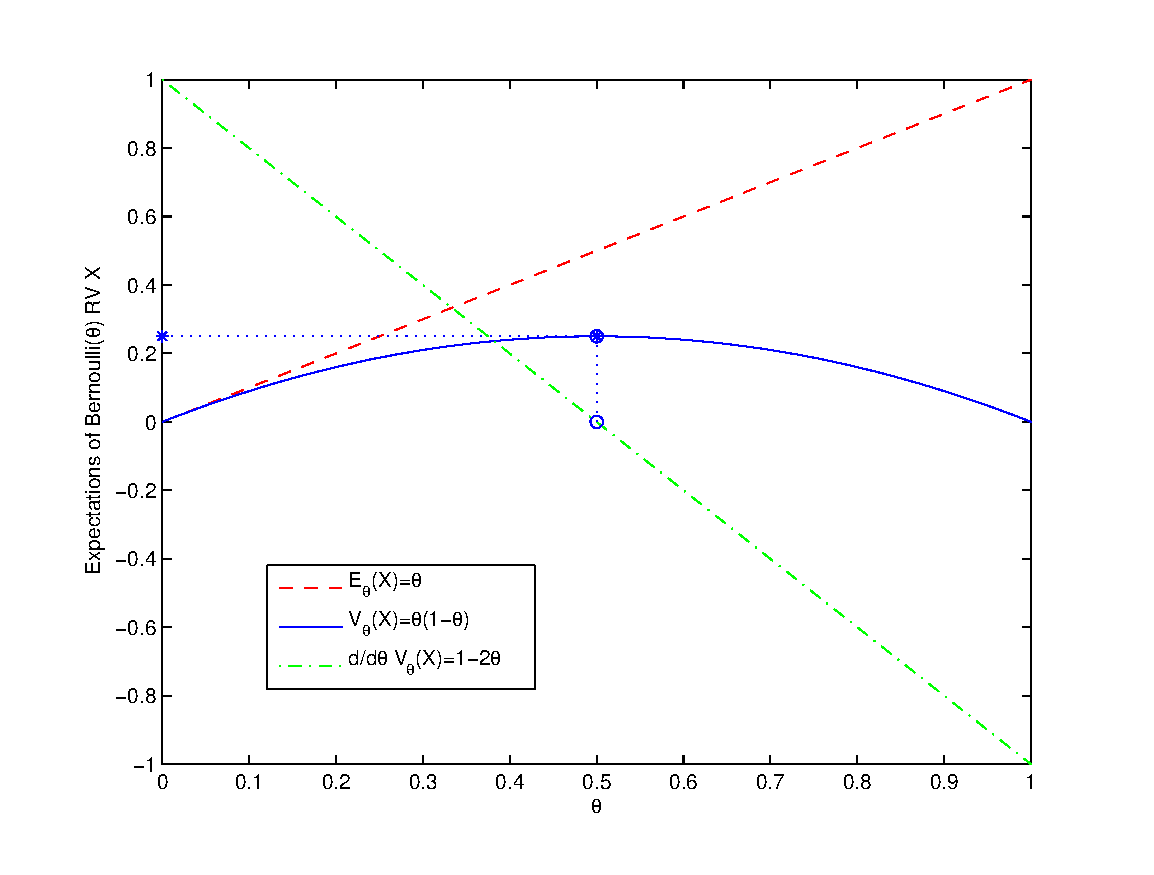
\includegraphics[width=5.0in]{figures/PlotMeanVarBernoulli}}
\end{figure}

Maximum of the variance $\V_{\theta}(X)$ is found by setting the derivative to zero, solving for $\theta$ and showing the second derivative is locally negative, i.e.~$\V_{\theta}(X)$ is concave down:
\[
\V_{\theta}'(X) := \frac{d}{d \theta} \V_{\theta}(X) = 1-2 \theta = 0  \iff \theta = \frac{1}{2} \ , 
\qquad \V_{\theta}''(X) := \frac{d}{d \theta} \left( \frac{d}{d \theta} \V_{\theta}(X) \right) = -2 < 0 \ ,
\]
\[
\max_{\theta \in [0,1]} \V_{\theta}(X) = \frac{1}{2} \left(1-\frac{1}{2} \right) = \frac{1}{4} \ , 
\text{since $\V_{\theta}(X)$ is maximized at $\theta = \frac{1}{2}$}
\]
The plot depicting these expectations as well as the rate of change of the variance are depicted in \hyperref[F:MeanVarBernoulli]{Figure \ref*{F:MeanVarBernoulli}}.  Note from this Figure that $\V_{\theta}(X)$ attains its maximum  value of $1/4$ at $\theta=0.5$ where $\frac{d}{d\theta}\V_{\theta}(X)=0$.  Furthermore, we know that we don't have a minimum at $\theta=0.5$ since the second derivative $\V_{\theta}''(X) = -2$ is negative for any $\theta \in [0,1]$.  This confirms that $\V_{\theta}(X)$ is concave down and therefore we have a maximum of $\V_{\theta}(X)$ at $\theta=0.5$.  We will revisit this example when we employ a numerical approach called Newton-Raphson method to solve for the maximum of a differentiable function by setting its derivative equal to zero.

\paragraph{Mean and variance of $\uniform(0,1)$ RV:}
Let $X \sim \uniform(0,1)$.  Then, 
\[
\e(X) = \int_{x=0}^1 x f(x)\, dx = \int_{x=0}^1 x \ 1 \, dx = \frac{1}{2} \left( x^2 \right]_{x=0}^{x=1} = \frac{1}{2} \left( 1-0 \right) = \frac{1}{2} \ ,
\]
\[
\e(X^2) = \int_{x=0}^1 x^2 f(x)\, dx = \int_{x=0}^1 x^2 \ 1 \, dx =  \frac{1}{3} \left( x^3 \right]_{x=0}^{x=1} = \frac{1}{3} \left( 1-0 \right) = \frac{1}{3} \ ,
\]
\[
\V(X) = \e(X^2) - (\e(X))^2 = \frac{1}{3}  - \left( \frac{1}{2} \right)^2  = \frac{1}{3}  - \frac{1}{4} = \frac{1}{12} \ .
\]

\begin{example}[Expected Exponential of the $Uniform(0,1)$ RV]
Let $X \sim Uniform(0,1)$ and $Y=r(X)=e^X$.  Compute $\e(Y)$. 

We can simply apply the definition of $\e(r(X))$, since $Y=r(X)$, is just a function of $X$, as follows: 
\[
\e(Y) = \int_0^1 e^x f(x) dx = \int_0^1 e^x 1 \ dx = e-1 \ .
\]
%You could have also found out that the density $f(y)=1/y$ for the RV $Y$, provided $1<y<e$, and $0$ otherwise.  Again,
%\[
%\e(Y) = \int_1^e y f(y) dy = \int_1^e y \frac{1}{y} dy = \int_1^e 1 \ dy = e-1 \ .
%\]
\end{example}

\paragraph{Mean and Variance of $\exponential(\lambda)$:}
Show that the mean of an $\exponential(\lambda)$ RV $X$ is:
\[
\e_{\lambda}(X) = \int_{0}^{\infty} x f(x;\lambda)\,dx
=   \int_{0}^{\infty} x \lambda e^{-\lambda x}\,dx
= \frac{1}{\lambda} \ ,
\]
and the variance is:
\[
\V_{\lambda}(X) = \left(  \frac{1}{\lambda} \right)^2 \ .
\]


\section{Stochastic Processes}\label{S:StochProc}

\begin{definition}[Stochastic Process]
A collection of RVs  \[
\left(X_{\alpha} \right)_{\alpha \in N} := \left( \  X_{\alpha} : \alpha \in \Az \  \right)
\]
is called a {\bf stochastic process}.  Thus, for every $\alpha \in  \Az$, the index set of the stochastic process, $X_{\alpha}$ is a RV.  If the index set $ \Az  \subset \Zz$ then we have  a {\bf discrete time stochastic process}, typically denoted by 
\[
\left(X_i\right)_{i \in \Zz} := \ldots, X_{-2},X_{-1},X_0, X_1,X_2,\ldots , \  \text{or}
\]
\[
\left( X_i \right)_{i \in \Nz} := X_1,X_2,\ldots , \  \text{or}
\]
\[
\left( X_i \right)_{i \in [n]} := X_1,X_2,\ldots , X_n , \ \text{where, } [n]:= \{1,2,\ldots,n\} \ .
\]
If $\Az \subset \Rz$ then we have a {\bf continuous time stochastic process}, typically denoted by $\{X_t\}_{t \in \Rz}$, etc.  
\end{definition}

\begin{definition}[Independent and Identically Distributed (IID)]
The finite or infinite sequence of RVs or the stochastic process $X_1, X_2,\ldots$ is said to be independent and identically distributed or IID if :
\begin{itemize}
\item they are an idependently distributed according to \hyperref[D:IndRVs]{Definition \ref*{D:IndRVs}}, and
\item $F(X_1) = F(X_2) = \cdots $, ie.~all the $X_i$'s have the same DF $F(X_1)$.
\end{itemize}
This is perhaps the most elementary class of stochastic processes and we succinctly denote it by
\[
\left(X_i\right)_{i \in [n]} := X_1, X_2,\ldots, X_n \overset{\IID}{\sim} F, \quad \text{or} \quad \left(X_i\right)_{i \in \Nz} := X_1, X_2,\ldots  \overset{\IID}{\sim} F \ .
\]
We sometimes replace the DF $F$ above by the name of the RV.
 \end{definition}
 
\begin{definition}[Independently Distributed]
The sequence of RVs or the stochastic process $\left(X_i\right)_{i \in \Nz} := X_1, X_2,\ldots$ is said to be independently distributed if :
\begin{itemize}
\item $X_1, X_2,\ldots$ is independently distributed according to \hyperref[D:IndRVs]{Definition \ref*{D:IndRVs}}.
\end{itemize}
This is a class of stochastic processes that is more general than the IID class.
\end{definition}

